\documentclass[11pt]{article}

%Standard Stefanos Packages
\usepackage[utf8]{inputenc}
\usepackage{dirtytalk}
\usepackage{amsmath}
\usepackage{mathtools}  
\mathtoolsset{showonlyrefs} 
\usepackage{graphicx}
\usepackage{mdframed}
\usepackage{lipsum}
\usepackage{cancel}
\usepackage{systeme}
\usepackage{pgfplots}
\usepackage{textcomp}
\usepackage{geometry}
\usetikzlibrary{arrows}
\geometry{a4paper}
\graphicspath{ {./res/} }
\usepackage{float}
\restylefloat{table}
\newcommand{\comment}[1]{%
	\text{\phantom{(#1)}} \tag{#1}
}
\usepackage{enumitem}% http://ctan.org/pkg/enumitem
\usepackage{physics}
\usepackage{subcaption}
\usepackage{graphicx}
\title{\line(1,0){450}\\ CS3DS19 - Data Science Algorithms and Tools \\ \large{Major Coursework }  \\\line(1,0){450} \\2021/2022}
\usepackage{pgfplots}
\author{Student ID: 27020363}
\newmdtheoremenv{note}{Note}
\pgfplotsset{compat=1.17}

%Extra Packages
\usepackage{tikz}
\usetikzlibrary{automata,positioning}

\usepackage{listings}
\usepackage{xcolor}

\definecolor{dkgreen}{rgb}{0,0.6,0}
\definecolor{gray}{rgb}{0.5,0.5,0.5}
\definecolor{mauve}{rgb}{0.58,0,0.82}

%line spacing
\usepackage{mathptmx}
\usepackage{setspace}
\setstretch{1.15}

%ms word
\setlength{\oddsidemargin}{0.0cm} \setlength{\evensidemargin}{.0cm} \setlength{\textwidth}{17cm} \setlength{\topmargin}{-1.50cm} \setlength{\textheight}{25cm} \setlength{\footskip}{0.8cm}


\lstdefinestyle{myScalastyle}{
	frame=tb,
	language=scala,
	aboveskip=3mm,
	belowskip=3mm,
	showstringspaces=false,
	columns=flexible,
	basicstyle={\small\ttfamily},
	numbers=none,
	numberstyle=\tiny\color{gray},
	keywordstyle=\color{blue},
	commentstyle=\color{dkgreen},
	stringstyle=\color{mauve},
	frame=single,
	breaklines=true,
	breakatwhitespace=true,
	tabsize=3,
}
\begin{document}
	\maketitle
	\pagebreak
	
	\section*{Task 0: Exploratory Data Analysis}
		In this section, we will try to familiarise ourselves with the given dataset, with the ultimate goal of designing an appropriate pre-processing process necessary for our future workflows. It is noteworthy that a normalisation process is absent from our EDA; Normalisation will be explained and applied on Task 2.
		\subsection*{Missing values detection}
			The first part of EDA is the detection of possible Missing values. We used the 'statistics' node (output contains 'No of Missing' variable) and sum for all the variables by using 'Group By' Node. The results, along with the node configurations, are given below. Based on the findings, we can safely ignore a missing values pre-prepossessing step.
			\iftrue
			\begin{center}
				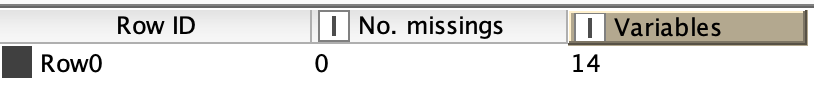
\includegraphics[scale=0.5]{res/t0/t01/t01-missing-values-res}
			\end{center}
			\fi
			\subsubsection*{Workflow and node configurations for missing values detection}
			\iftrue
			\begin{center}
				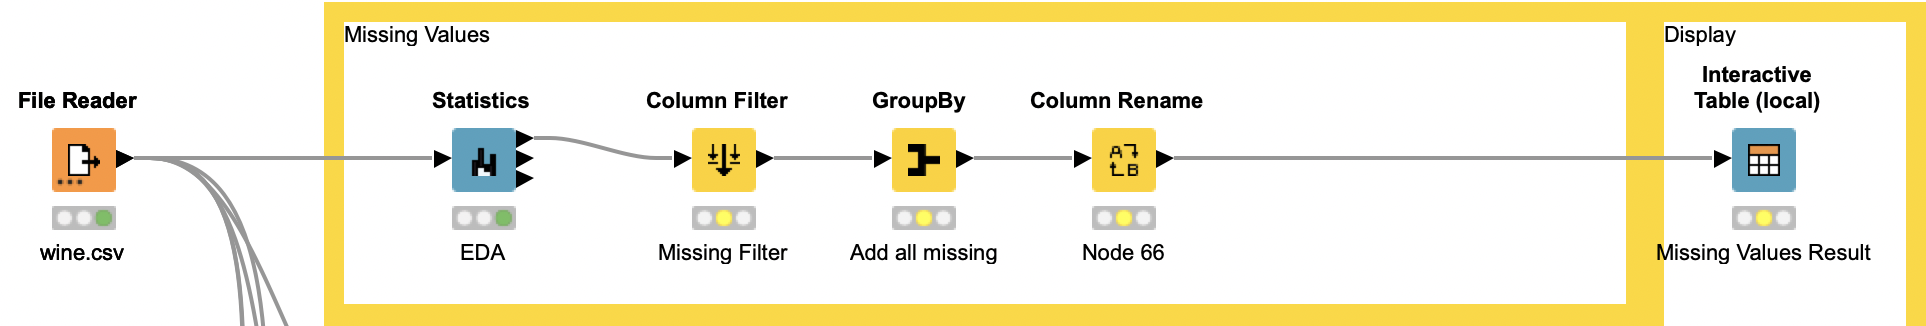
\includegraphics[scale=0.5]{res/t0/t01/t01-workflow}
			\end{center}
			\fi
			\iftrue
			\begin{figure}[H]
				\centering
				\begin{subfigure}{0.4\textwidth}
					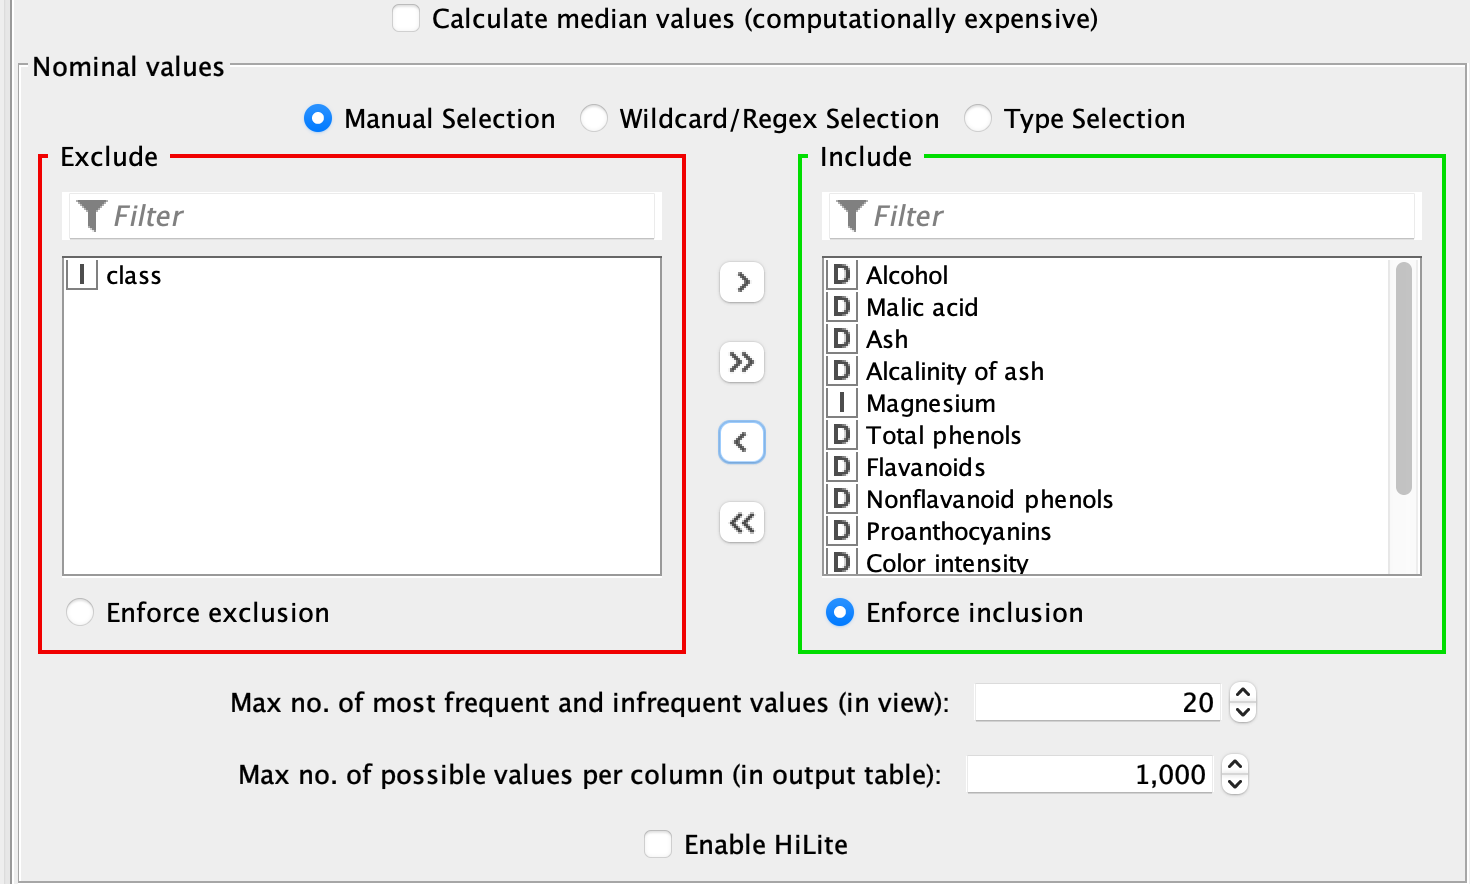
\includegraphics[width=\textwidth]{res/t0/t01/t01-statistics-conf}
					\caption{Statistics Node: Generate various statistics, 'Number of missing' per variable, variable included}
					\label{fig:first}
				\end{subfigure}
				\hfill
				\begin{subfigure}{0.4\textwidth}
					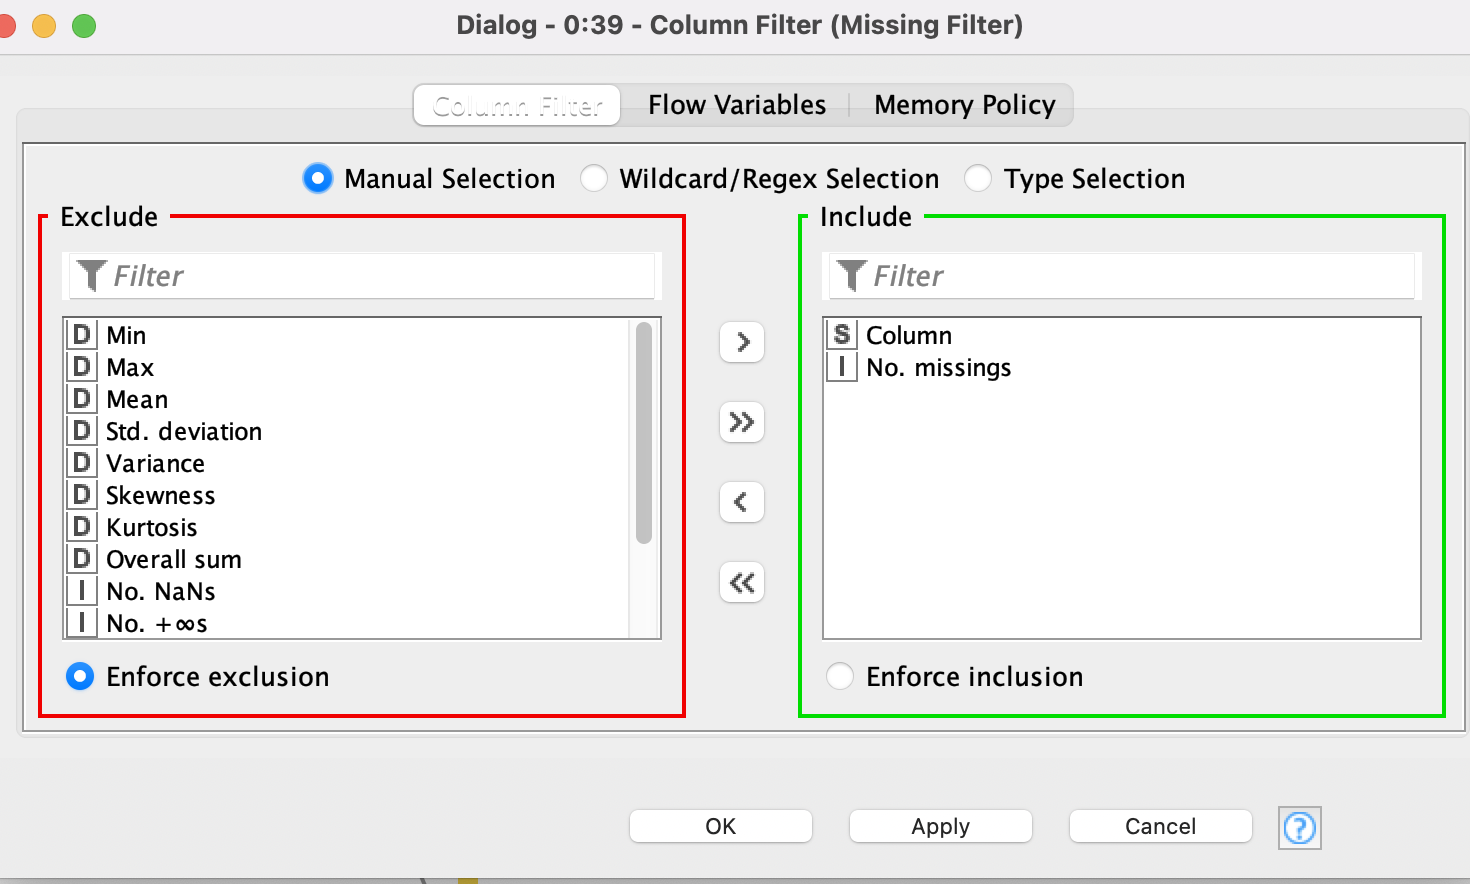
\includegraphics[width=\textwidth]{res/t0/t01/t01-column-filter-conf}
					\caption{Column Filter: Keep only 'No of Missing' and Variable Name}
					\label{fig:second}
				\end{subfigure}
				\hfill
				\begin{subfigure}{0.4\textwidth}
					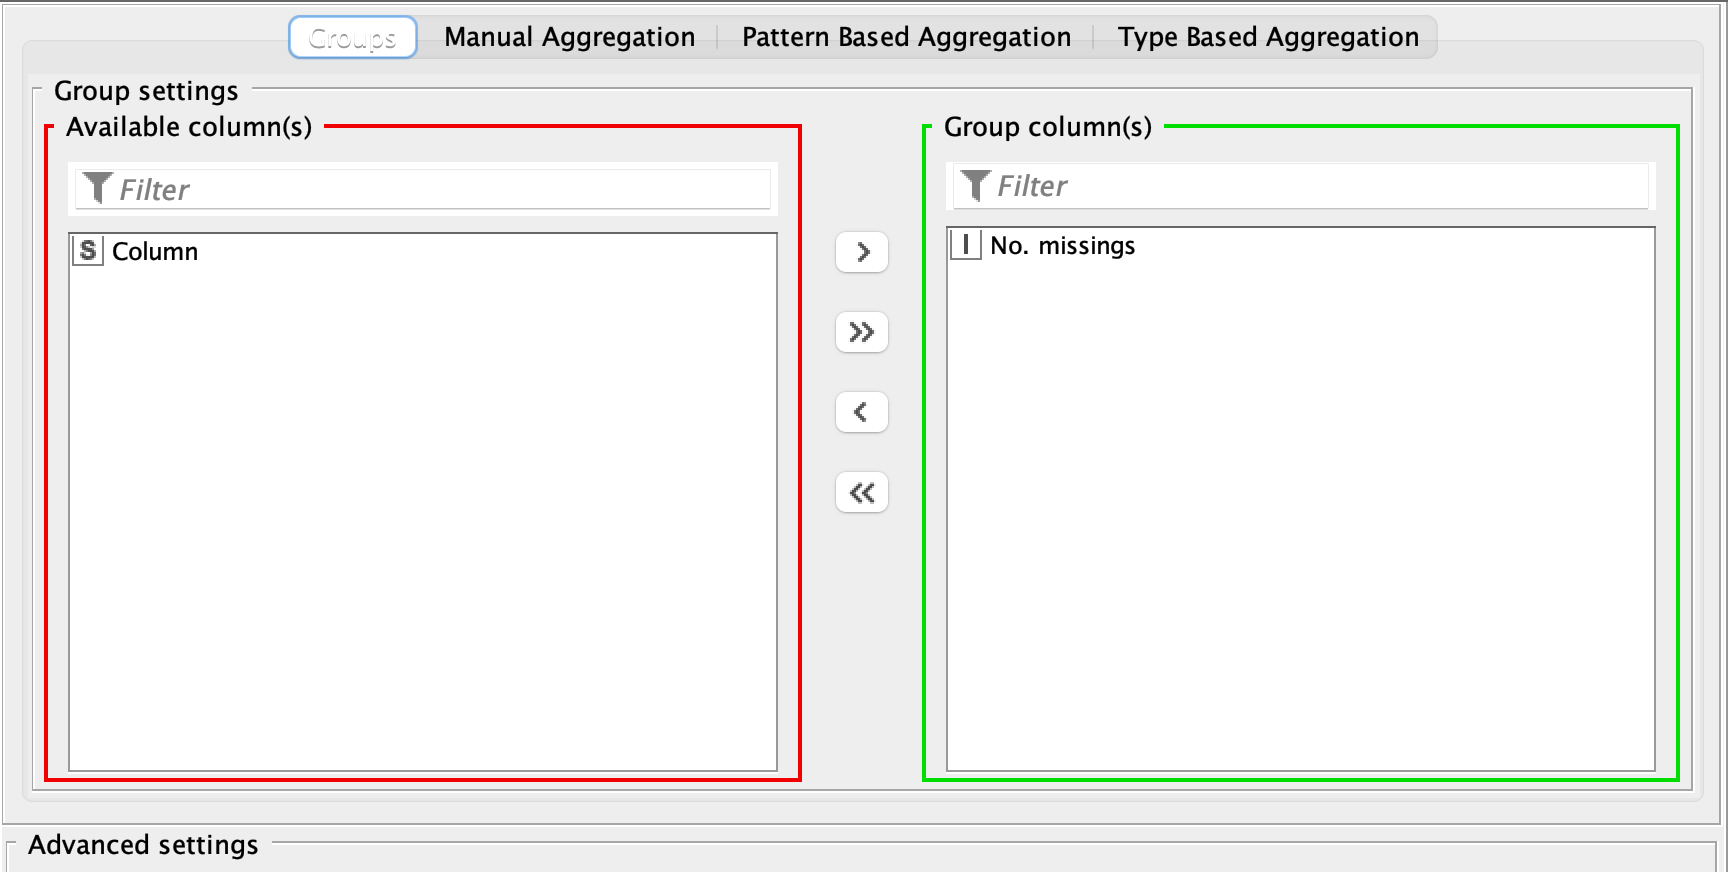
\includegraphics[width=\textwidth]{res/t0/t01/t01-groupby-conf-1}
					\caption{Reduce: Apply SUM function to 'No of Missing' per variable, groups}
					\label{fig:third}
				\end{subfigure}	
				\hfill
				\begin{subfigure}{0.4\textwidth}
					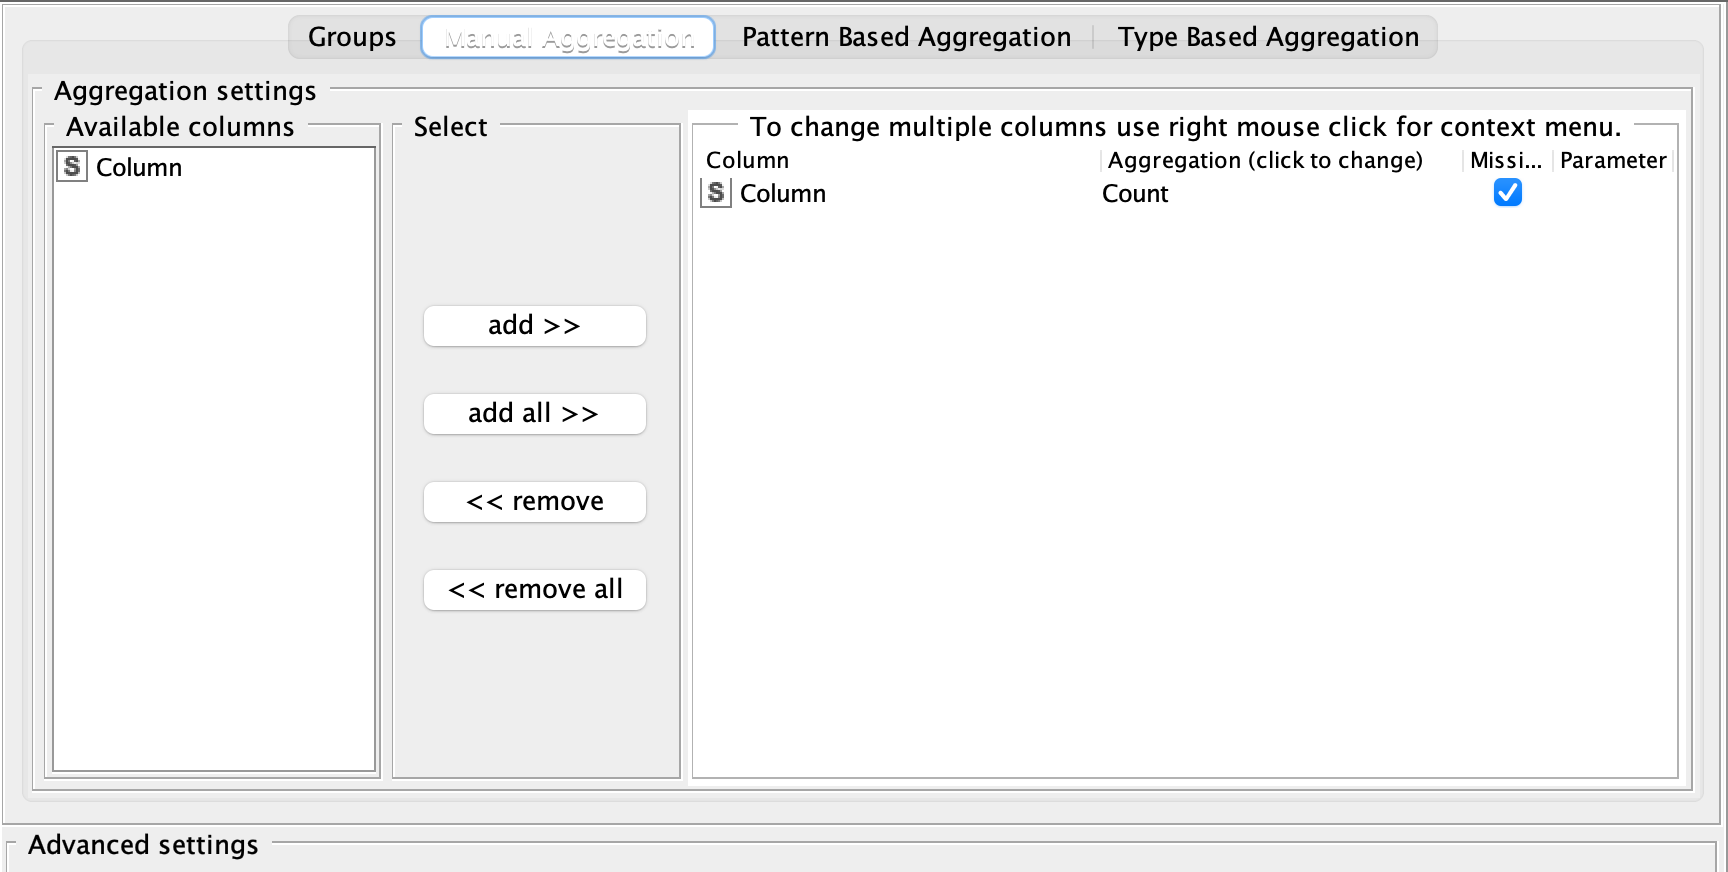
\includegraphics[width=\textwidth]{res/t0/t01/t01-groupby-conf-2}
					\caption{Reduce: Apply SUM function to 'No of Missing' per variable, aggregation}
					\label{fig:third}
				\end{subfigure}	
				\label{fig:figures}
			\end{figure}
			\fi
			
		\subsection*{Duplicate detection}
			The second part of EDA detects and removes duplicate rows from our dataset. Our logic is relatively simple, we applied a 'Duplicate Row Filter' into the dataset, and we counted the number of rows of this result. If the number of rows remains unchanged, we do not have duplicates. The results suggest that, indeed, there are no duplicate entries, so it's safe to ignore a duplicate filter as a pre-processing step.
			\iftrue
			\begin{center}
				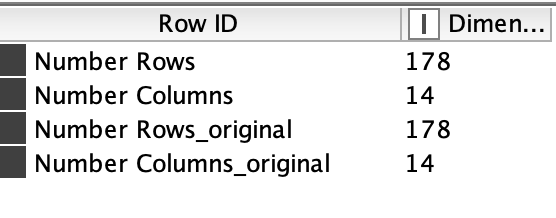
\includegraphics[scale=0.5]{res/t0/t02/t02-results}
			\end{center}
			\fi
			\subsubsection*{Workflow and node configurations for duplicate detection}
			\iftrue
			\begin{center}
				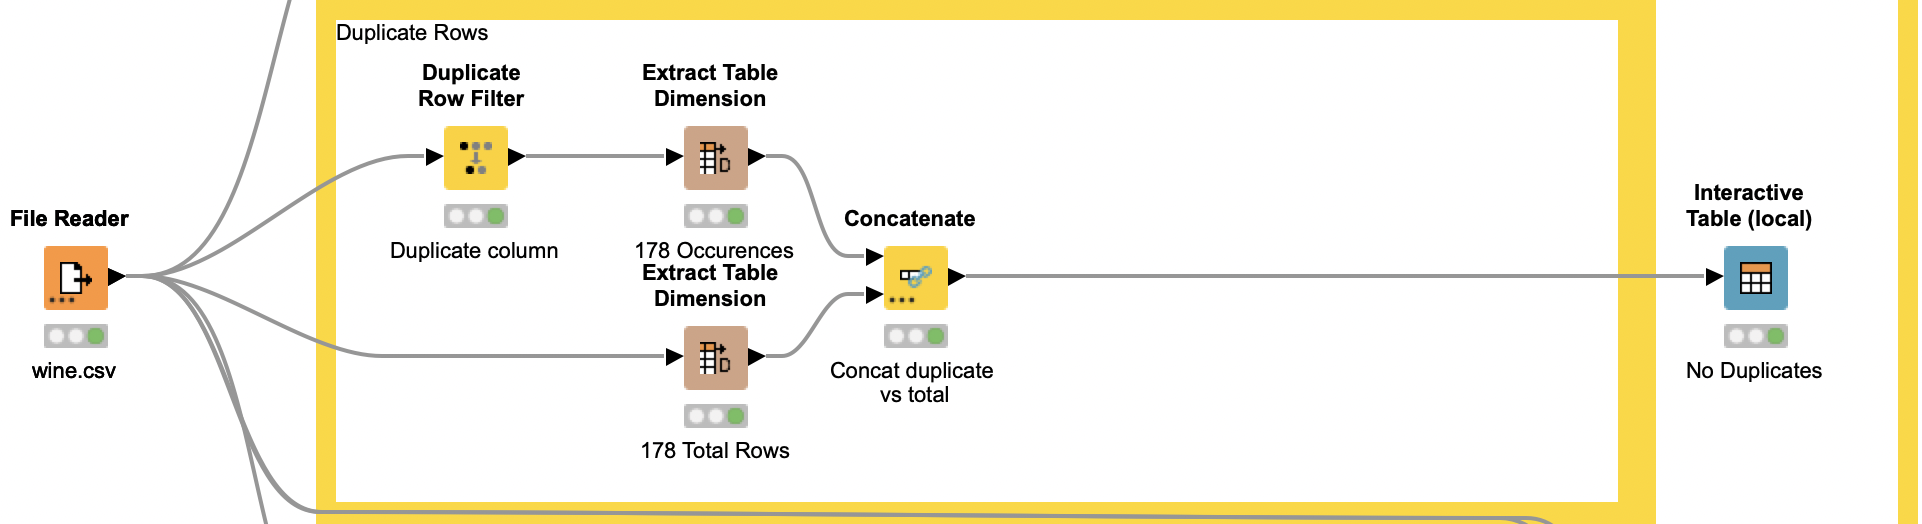
\includegraphics[scale=0.5]{res/t0/t02/t02-workflow}
			\end{center}
			\fi
			\iftrue
			\begin{figure}[H]
				\centering
				\begin{subfigure}{0.4\textwidth}
					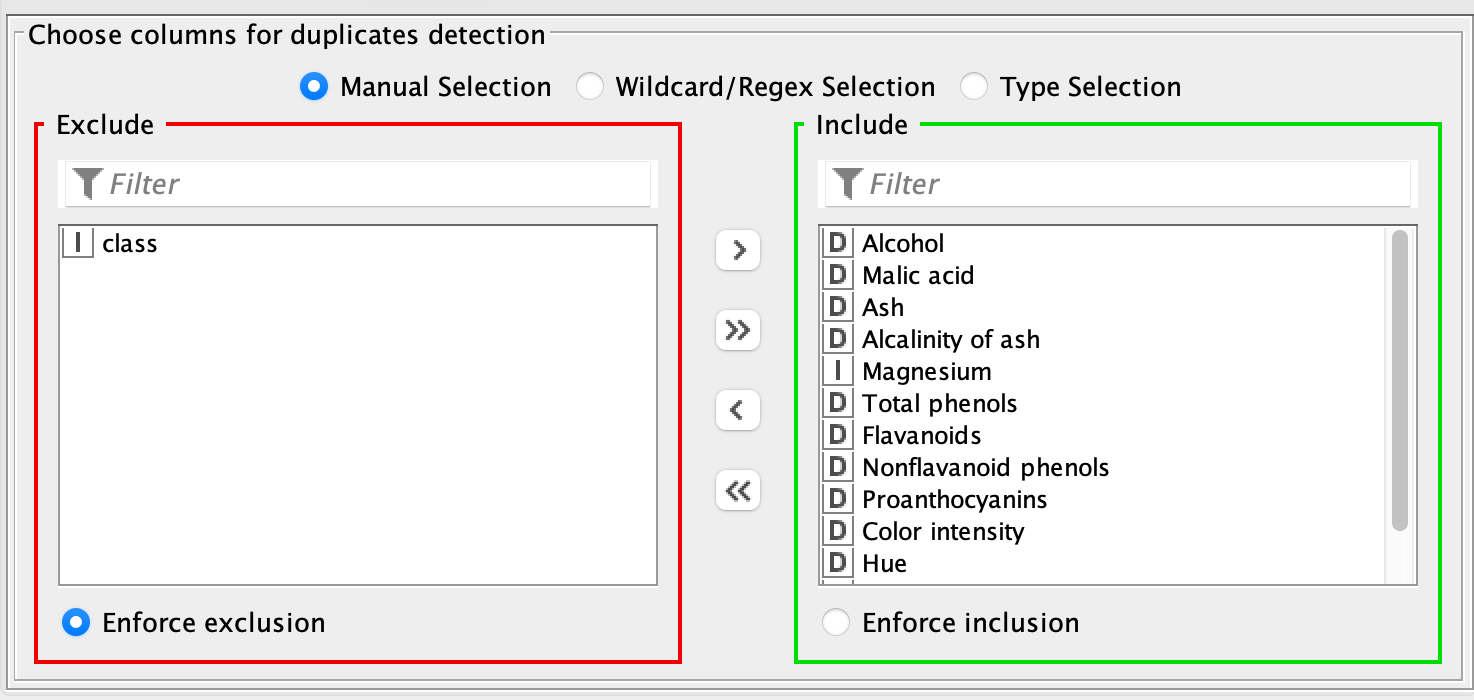
\includegraphics[width=\textwidth]{res/t0/t02/t02-duplicate-filter-conf}
					\caption{Duplicate row filter configuration}
					\label{fig:first}
				\end{subfigure}
				\hfill
				\begin{subfigure}{0.4\textwidth}
					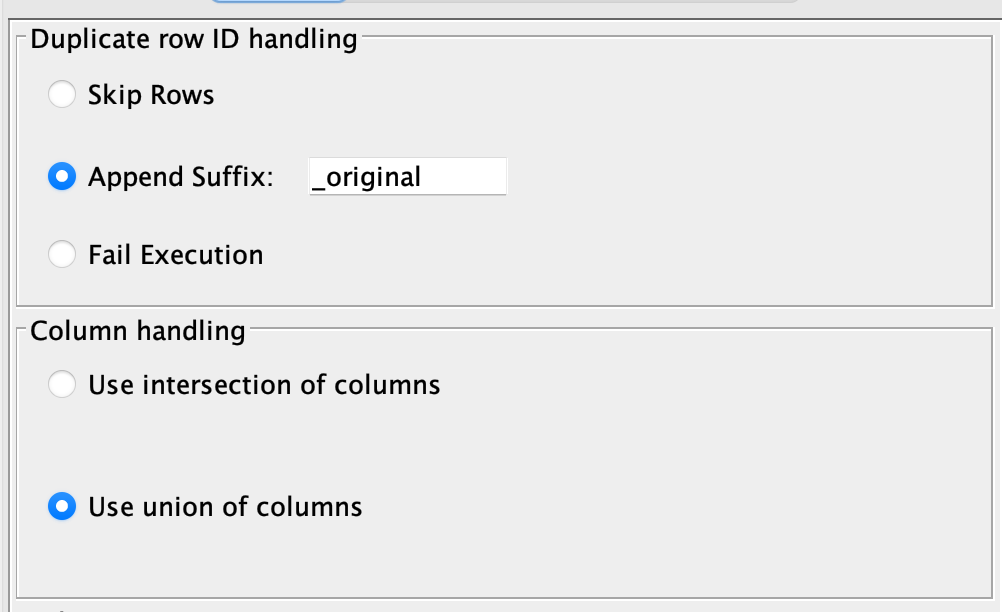
\includegraphics[width=\textwidth]{res/t0/t02/t02-concat-conf}
					\caption{Concatenation: We perform union on the table dimensions before and after removing the duplicates. If those numbers are equal, the filter removed 0 rows; hence there are no duplicates.}
					\label{fig:second}
				\end{subfigure}
				\hfill
			\end{figure}
			\fi
		\subsection*{Outliers detection}
			Our third part of our EDA contains the detection of outliers. We need to carefully think about outliers because of one of the limitations of our chosen clustering algorithm of choice. One of K-Means limitations are the sensitivity to outliers. \cite{k-means-sensitive}. 
			\subsubsection*{The process}
				Assuming an underlying approximate normal distribution on every one of our variables, we will use the famous 68-95-99 empirical rule\cite{3stddev-rule} to detect outliers. Part of the 68-95-99 rule states that $99.7\%$ of the data points in a given approximately normal distribution lies within the range $\mu \pm 3*\sigma$, where $\mu$ is the variable mean and $\sigma$ is the standard deviation. It is rather simple to detect outliers with the following method. We will use the output of the 'Statistics' node(columns 'max','min','mean','stddev'), and by using a simple mathematical formula, we can determine if, for a given variable, $\text{max}>\mu + 3\cdot\sigma$ or $\text{min}<\mu - 3\cdot\sigma$
			\subsubsection*{Results}
				The next figure displays the variables that may\footnote{because of our assumption of approximately normal distribution on our variables.} contain outliers.
				\iftrue
				\begin{center}
					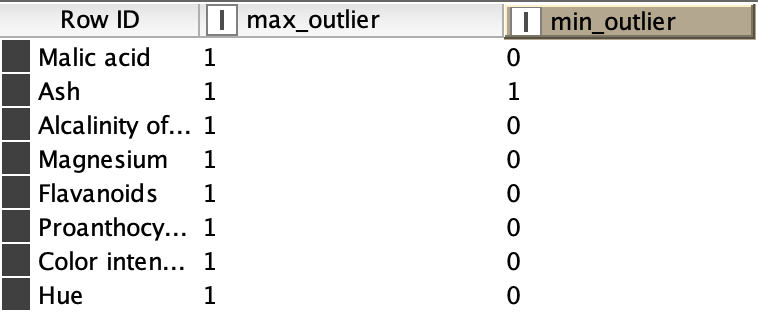
\includegraphics[scale=0.5]{res/t0/t03/t03-results}
				\end{center}
				\fi
				We can visualize those suspected variables with box plots to visually verify our findings.
				\iftrue
				\begin{figure}[H]
					\centering
					\begin{subfigure}{0.4\textwidth}
						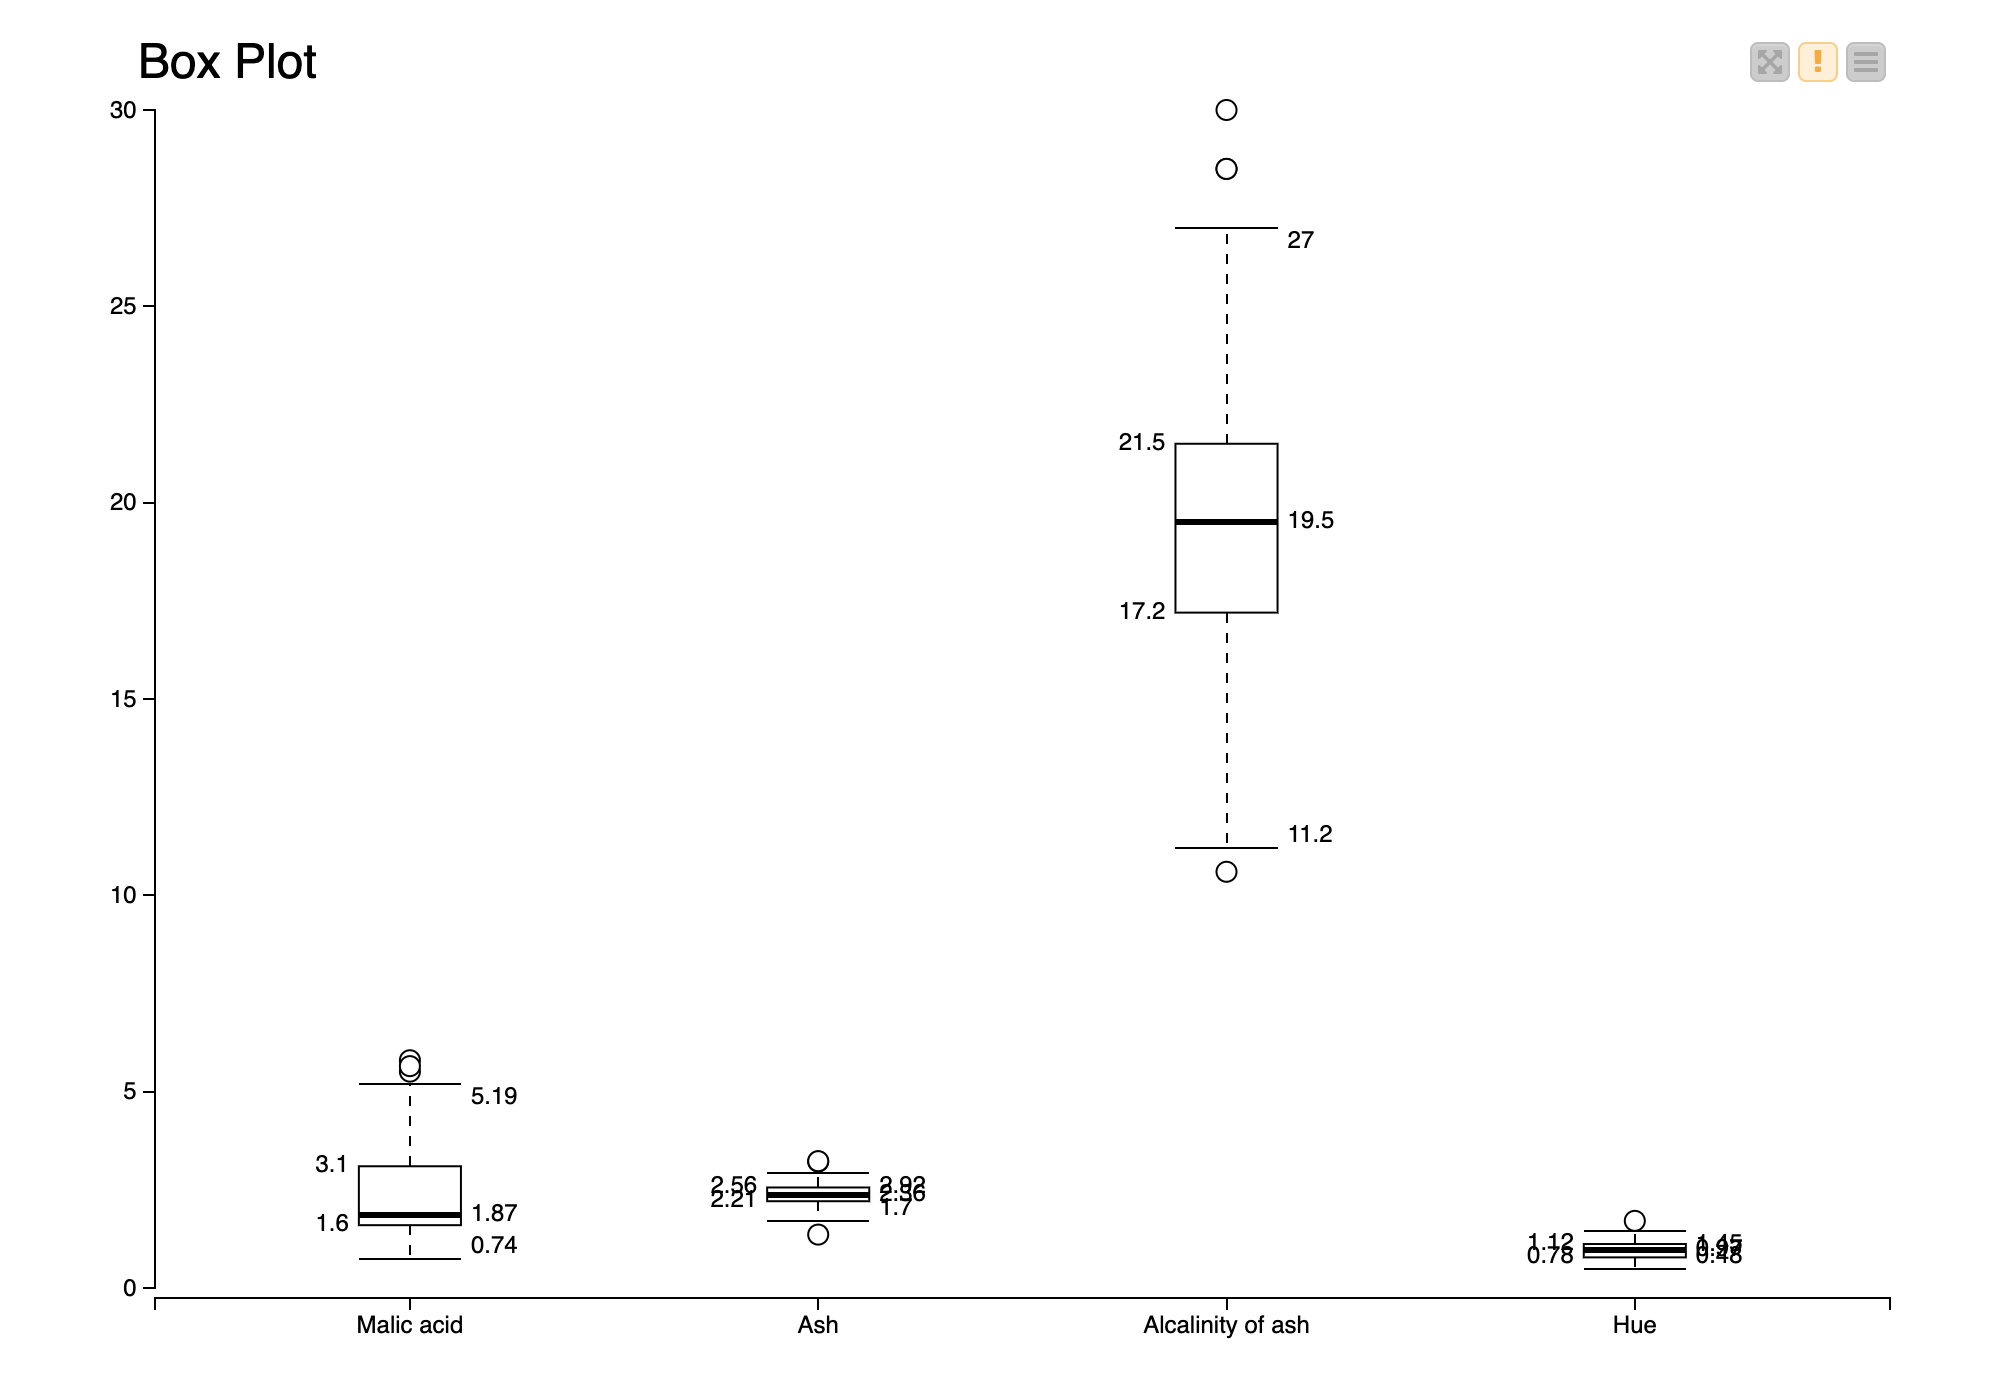
\includegraphics[width=\textwidth]{res/t0/t03/t03-results-box-plot-1}
						\caption{Malic acid - Ash - Alkalinity of ash - Magnesium}
						\label{fig:first}
					\end{subfigure}
					\hfill
					\begin{subfigure}{0.4\textwidth}
						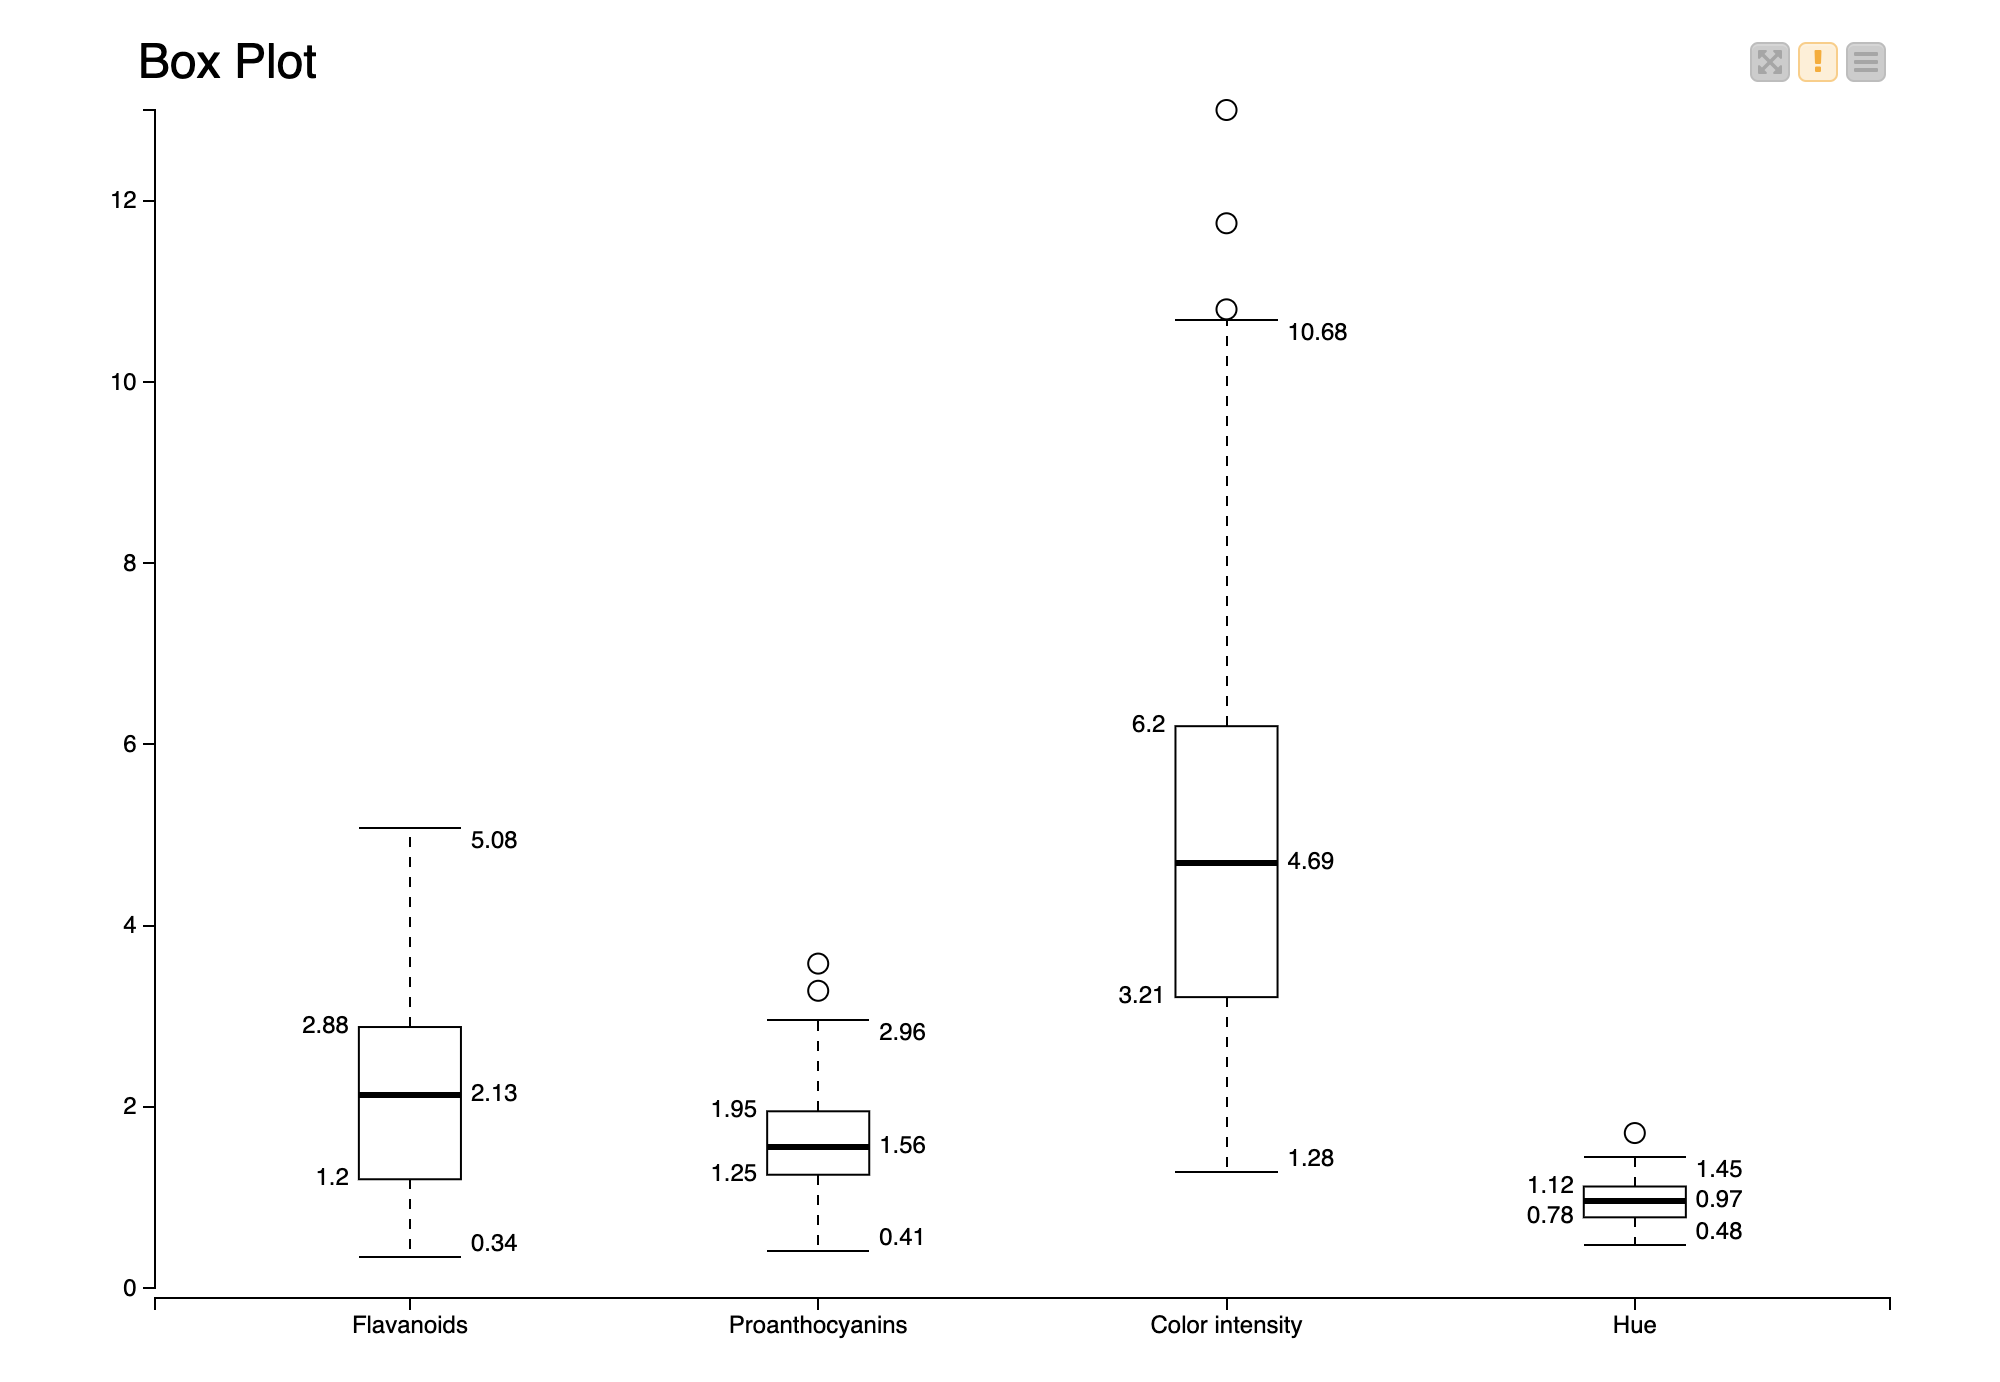
\includegraphics[width=\textwidth]{res/t0/t03/t03-results-box-plot-2}
						\caption{Flavanoids - Proanthocyanins - Color intensity - Hue}
						\label{fig:second}
					\end{subfigure}
					\hfill
				\end{figure}
				\fi
			\subsubsection*{Workflow and node configurations for outliers detection}
				\iftrue
				\begin{center}
					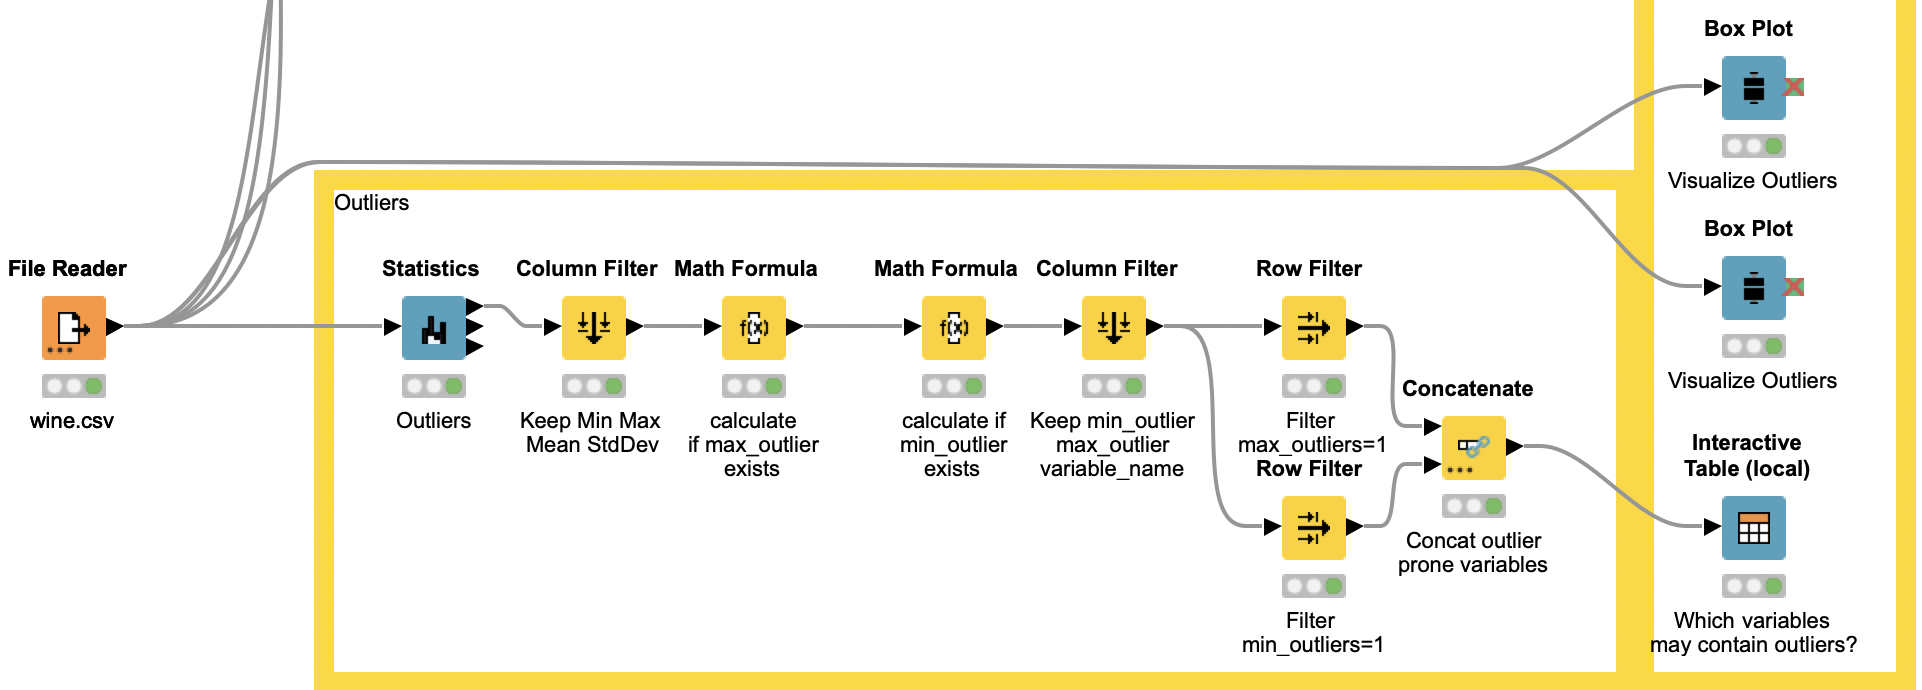
\includegraphics[scale=0.5]{res/t0/t03/t03-workflow}
				\end{center}
				\fi
				\iftrue
				\begin{figure}[H]
					\centering
					\begin{subfigure}{0.4\textwidth}
						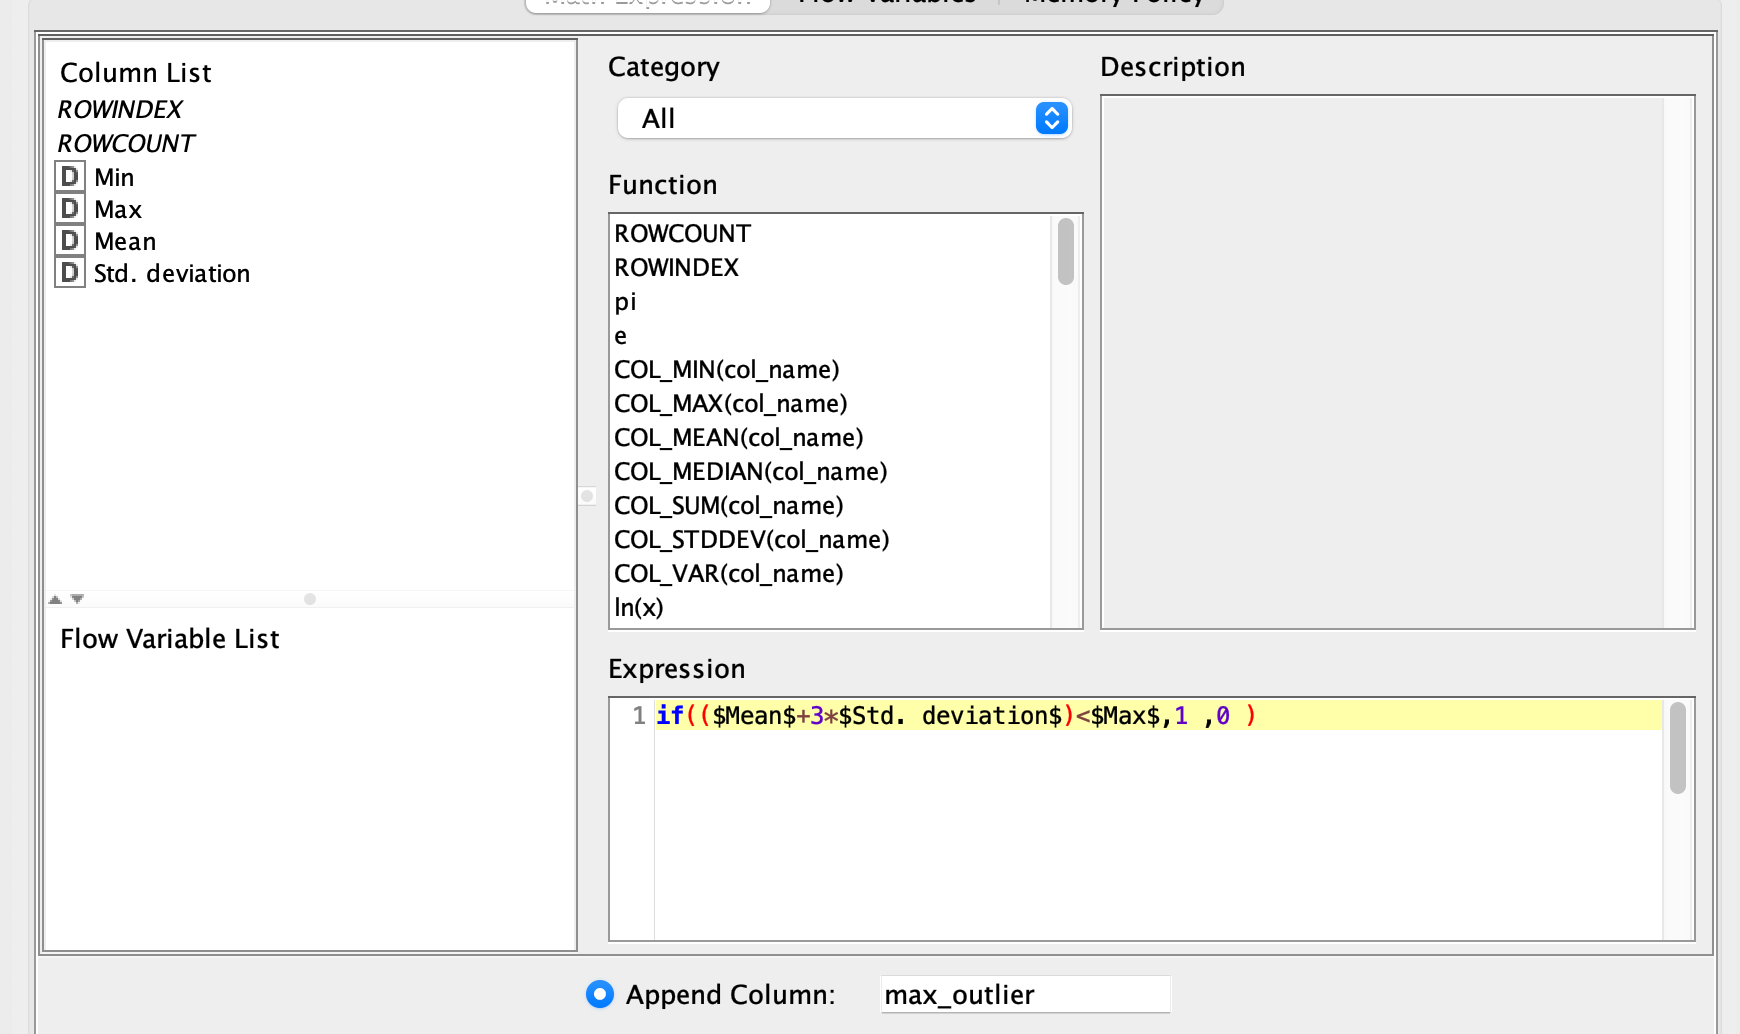
\includegraphics[width=\textwidth]{res/t0/t03/t03-math-formula-max-outliers-conf}
						\caption{We use the empirical rule to calculate if every variable's max exceeds $\mu + 3\cdot\sigma$}
						\label{fig:first}
					\end{subfigure}
					\hfill
					\begin{subfigure}{0.4\textwidth}
						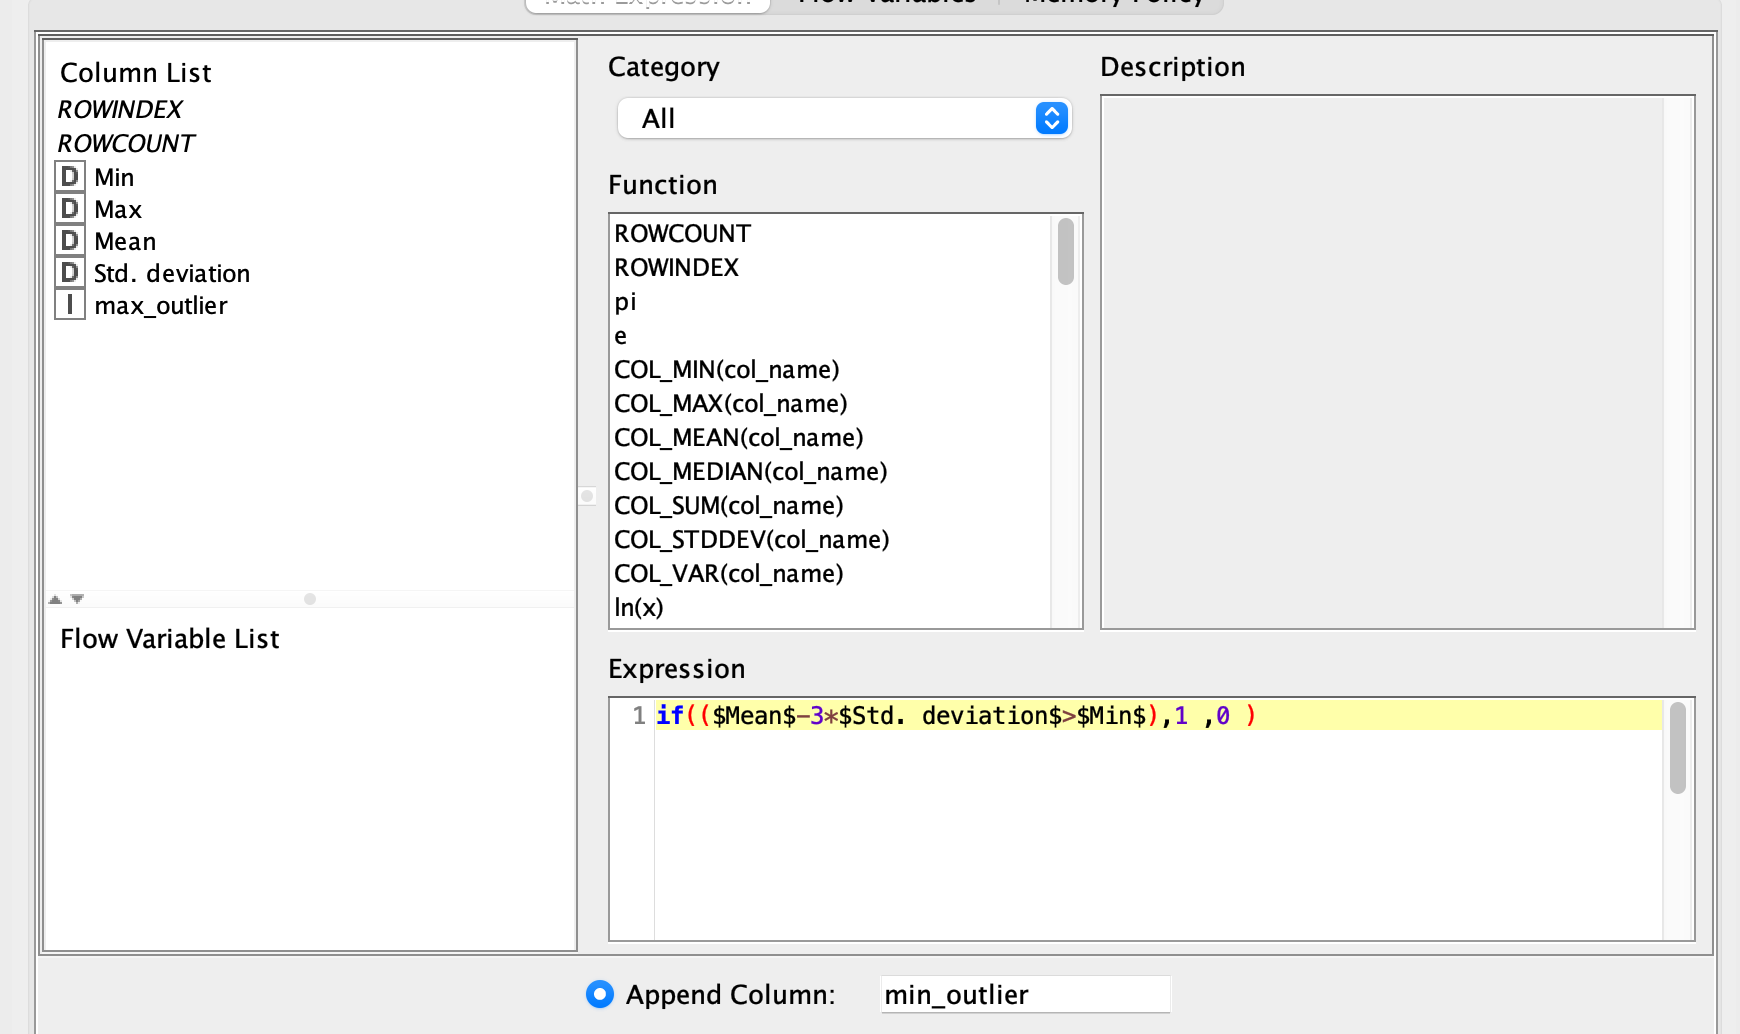
\includegraphics[width=\textwidth]{res/t0/t03/t03-math-formula-min-outliers-conf}
						\caption{We use the empirical rule again to calculate if every variable's min is smaller than $\mu - 3\cdot\sigma$}
						\label{fig:second}
					\end{subfigure}
					\hfill
					\begin{subfigure}{0.4\textwidth}
						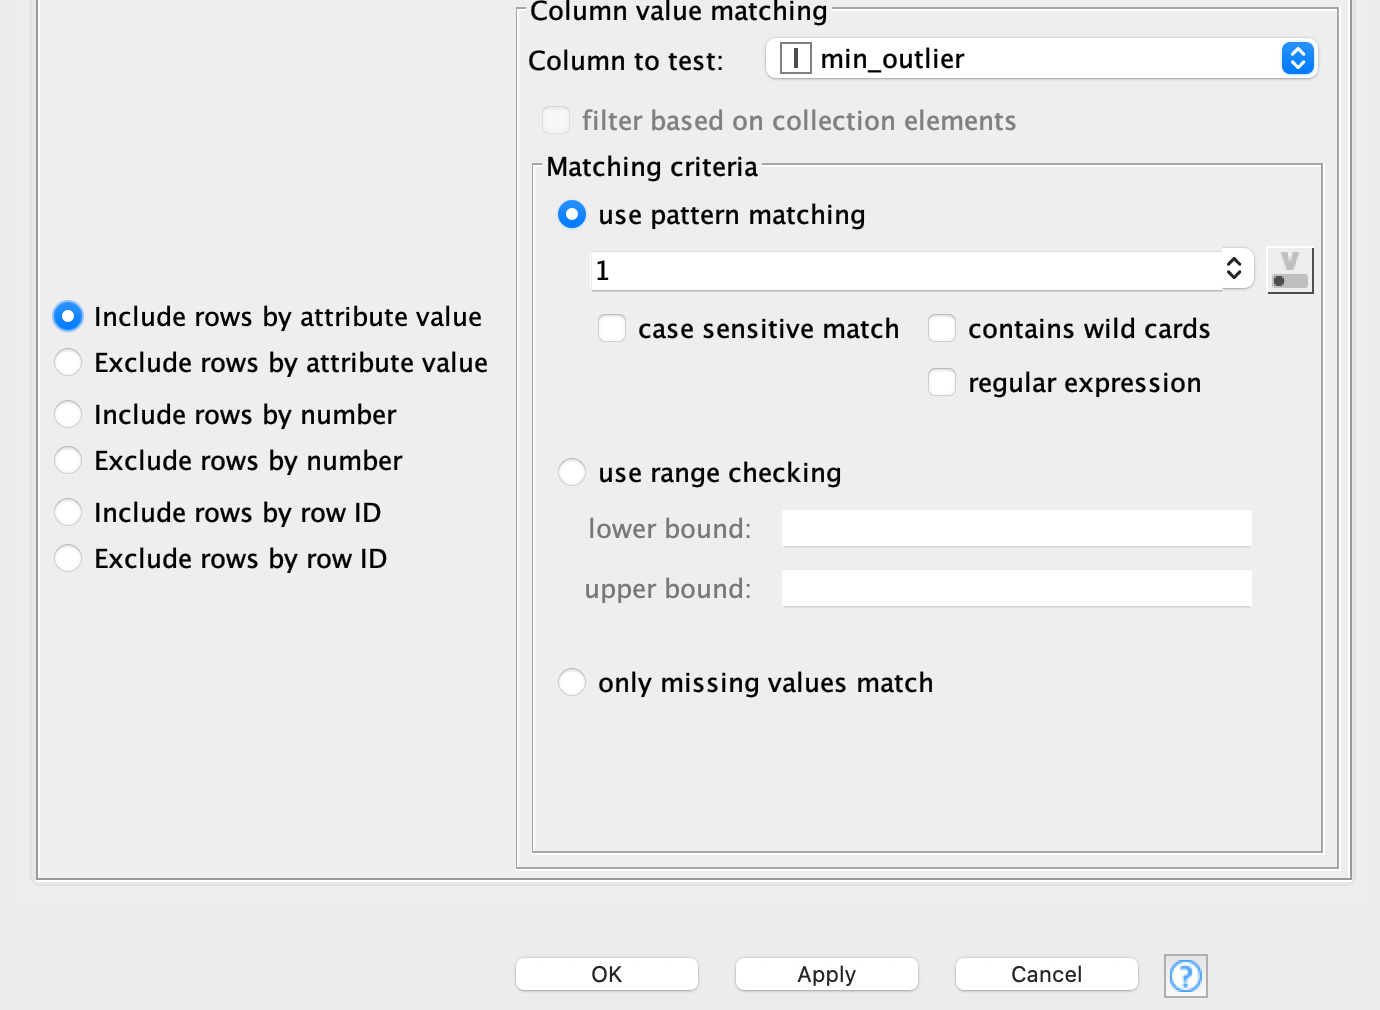
\includegraphics[width=\textwidth]{res/t0/t03/t03-min-outliers-filter-conf}
						\caption{Keep only the variables with min outliers(to be displayed later)}
						\label{fig:first}
					\end{subfigure}
					\hfill
					\begin{subfigure}{0.4\textwidth}
						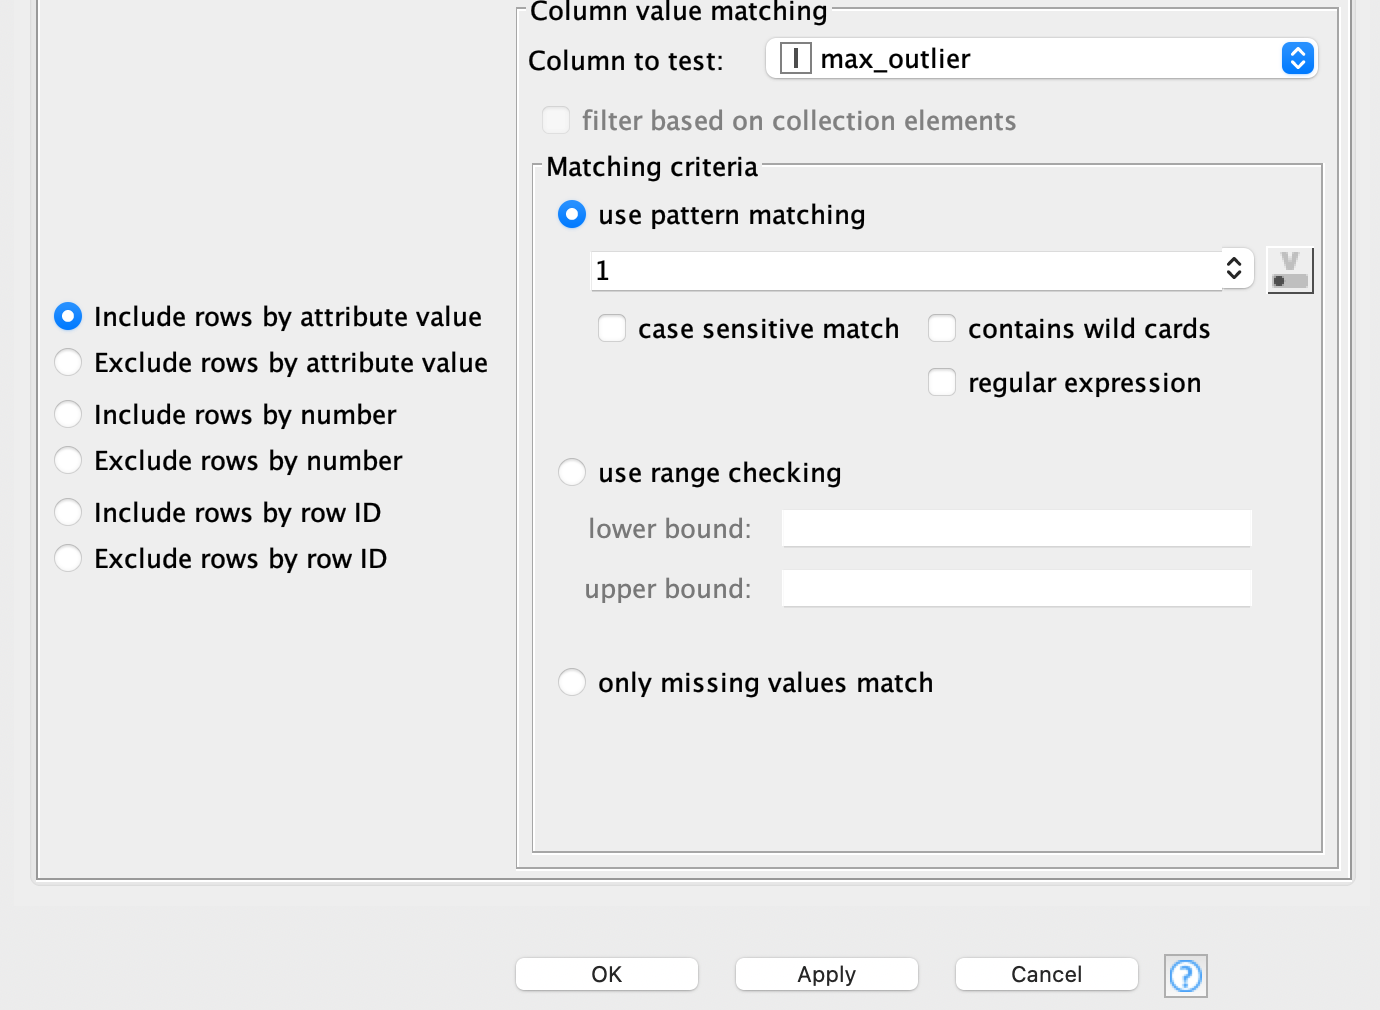
\includegraphics[width=\textwidth]{res/t0/t03/t03-max-outliers-filter-conf}
						\caption{Keep only the variables with max outliers(to be displayed later)}
						\label{fig:second}
					\end{subfigure}
					\hfill
				\end{figure}
				\fi
			
		\subsection*{'Class' to  string}
			The last step of our EDA is to transform the 'class' column, from an integer column, into a string column; this is essential to be handled as a categorical variable by the colour manager, PCA, normalization, etc. This can be easily achieved with the following small workflow.
			\iftrue
			\begin{center}
				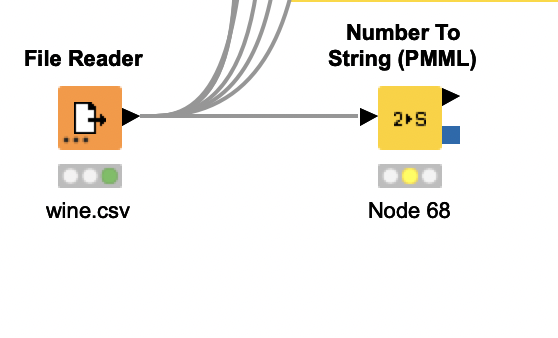
\includegraphics[scale=0.5]{res/t0/t04/t04-workflow}
			\end{center}
			\fi
			and the node configuration is given below
			\iftrue
			\begin{figure}[H]
				\centering
				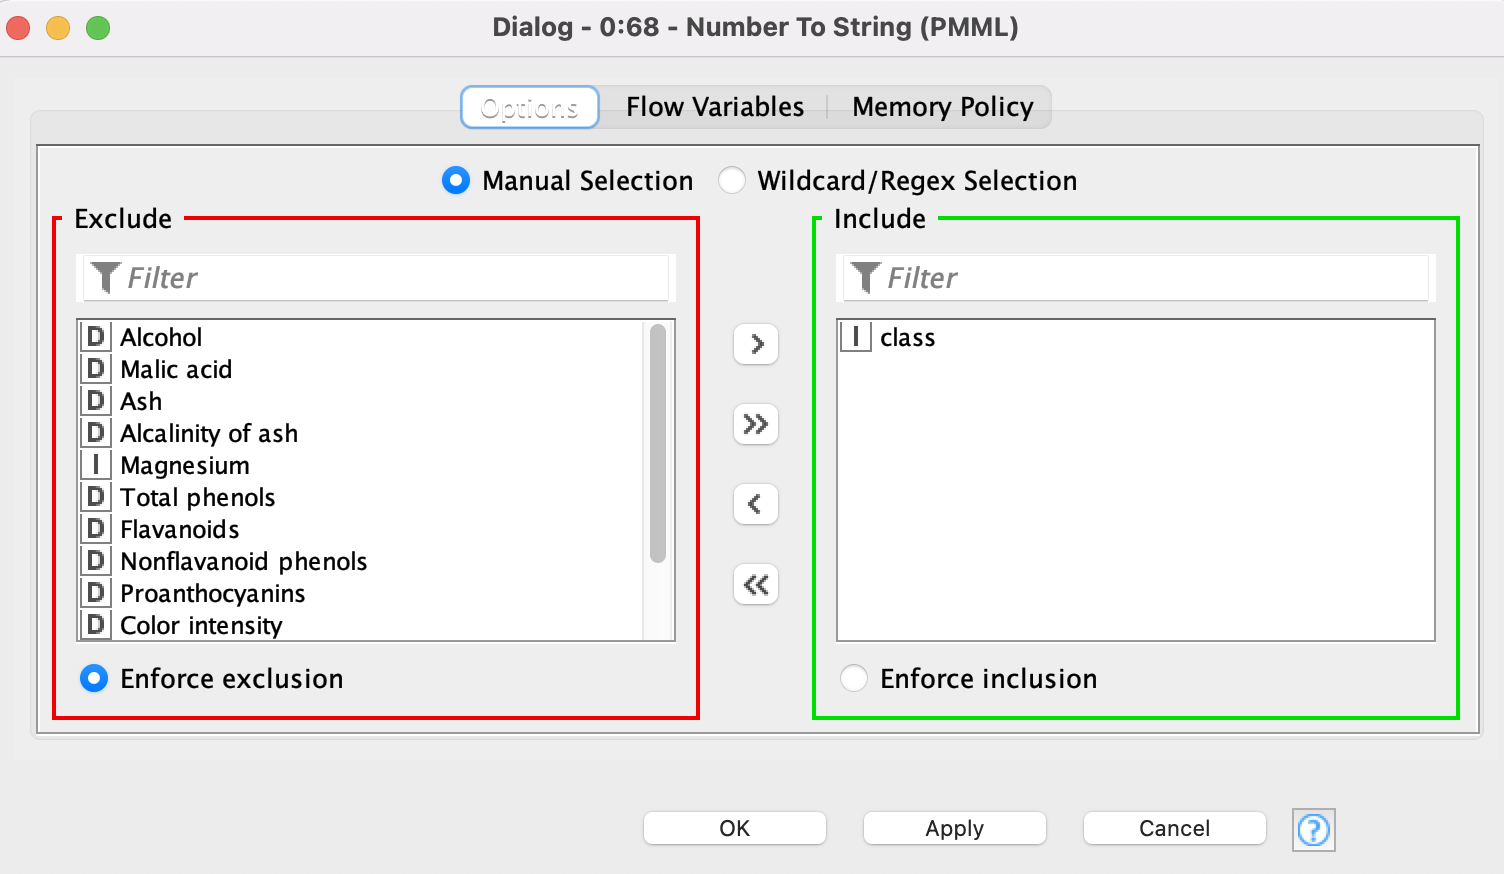
\includegraphics[scale=0.3]{res/t0/t04/t04-number-to-string-ppml-conf}
				\caption{Number to String PPML Node: Keep and transform only 'class' column}
				\label{fig:second}
			\end{figure}
			\fi
		\subsection*{Our Pre-processing strategy}
			Given our EDA, we now have a clear strategy for the initial data cleansing and processing. The following workflow will be transformed into a meta node and included in every workflow from now on. A noteworthy mention is that the 'numeric outliers' strategy is to remove the outlier rows.
			\iftrue
			\begin{center}
				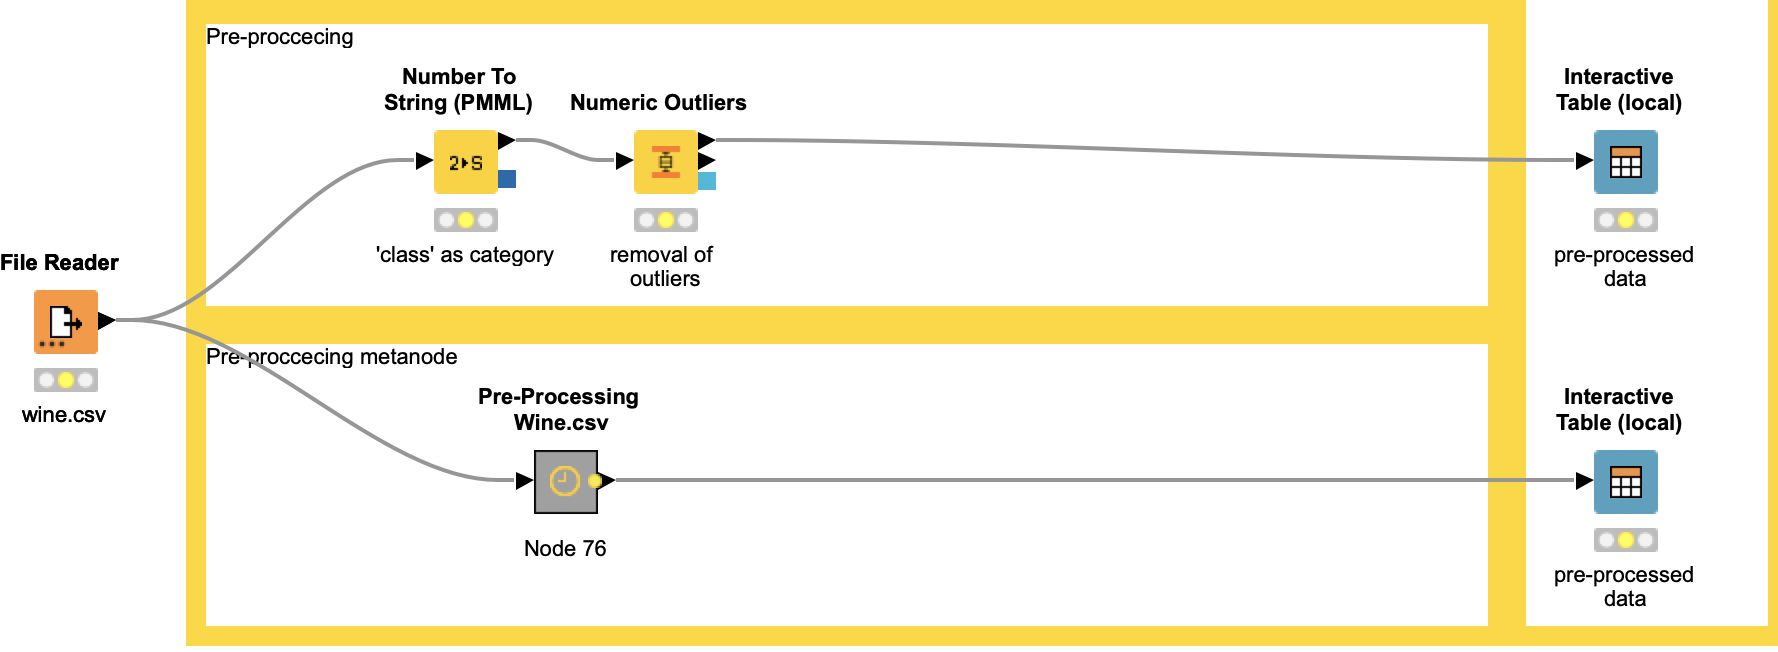
\includegraphics[scale=0.5]{res/t0/t05/t05-workflow}
			\end{center}
			\fi
			

	\section*{Task 1}
		\subsection*{Task 1.1 : Generate plot1}
			The workflow to generate plot1 is given below.
			\iftrue
			\begin{center}
				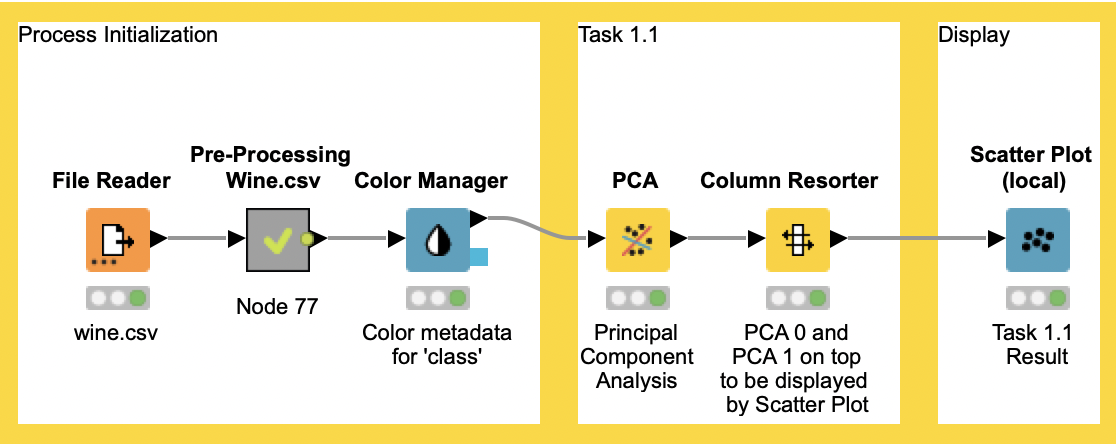
\includegraphics[scale=0.5]{res/t1/t11/t11-workflow}
			\end{center}
			\fi
			And the node configurations with descriptions are given below.
			\iftrue
			\begin{figure}[H]
				\centering
				\begin{subfigure}{0.4\textwidth}
					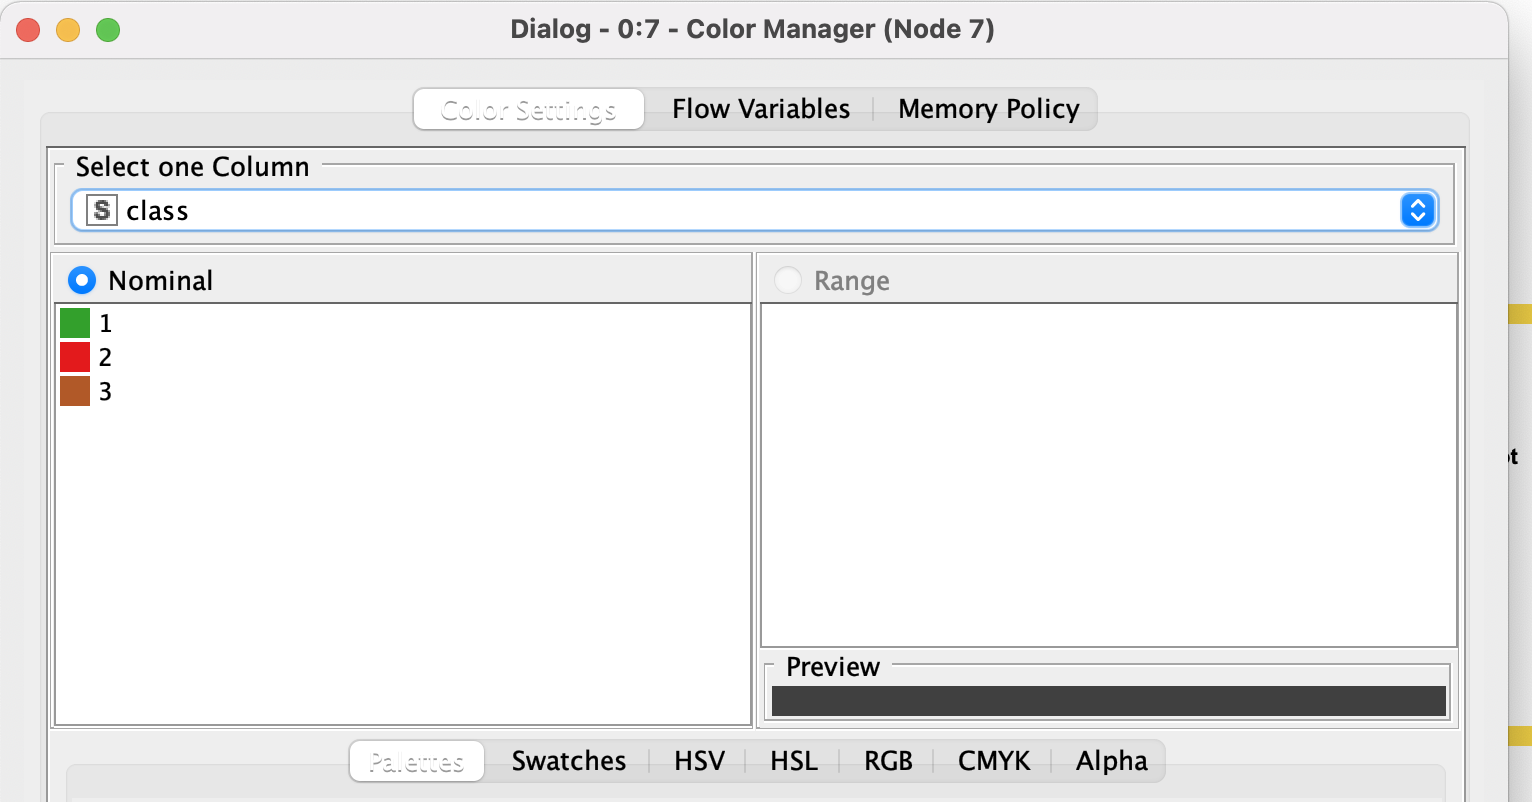
\includegraphics[width=\textwidth]{res/t1/t11/t11-color-manager-conf}
					\caption{Color Manager: Color Metadata for plot1 on 'class' column.}
					\label{fig:first}
				\end{subfigure}
				\hfil
				\begin{subfigure}{0.4\textwidth}
					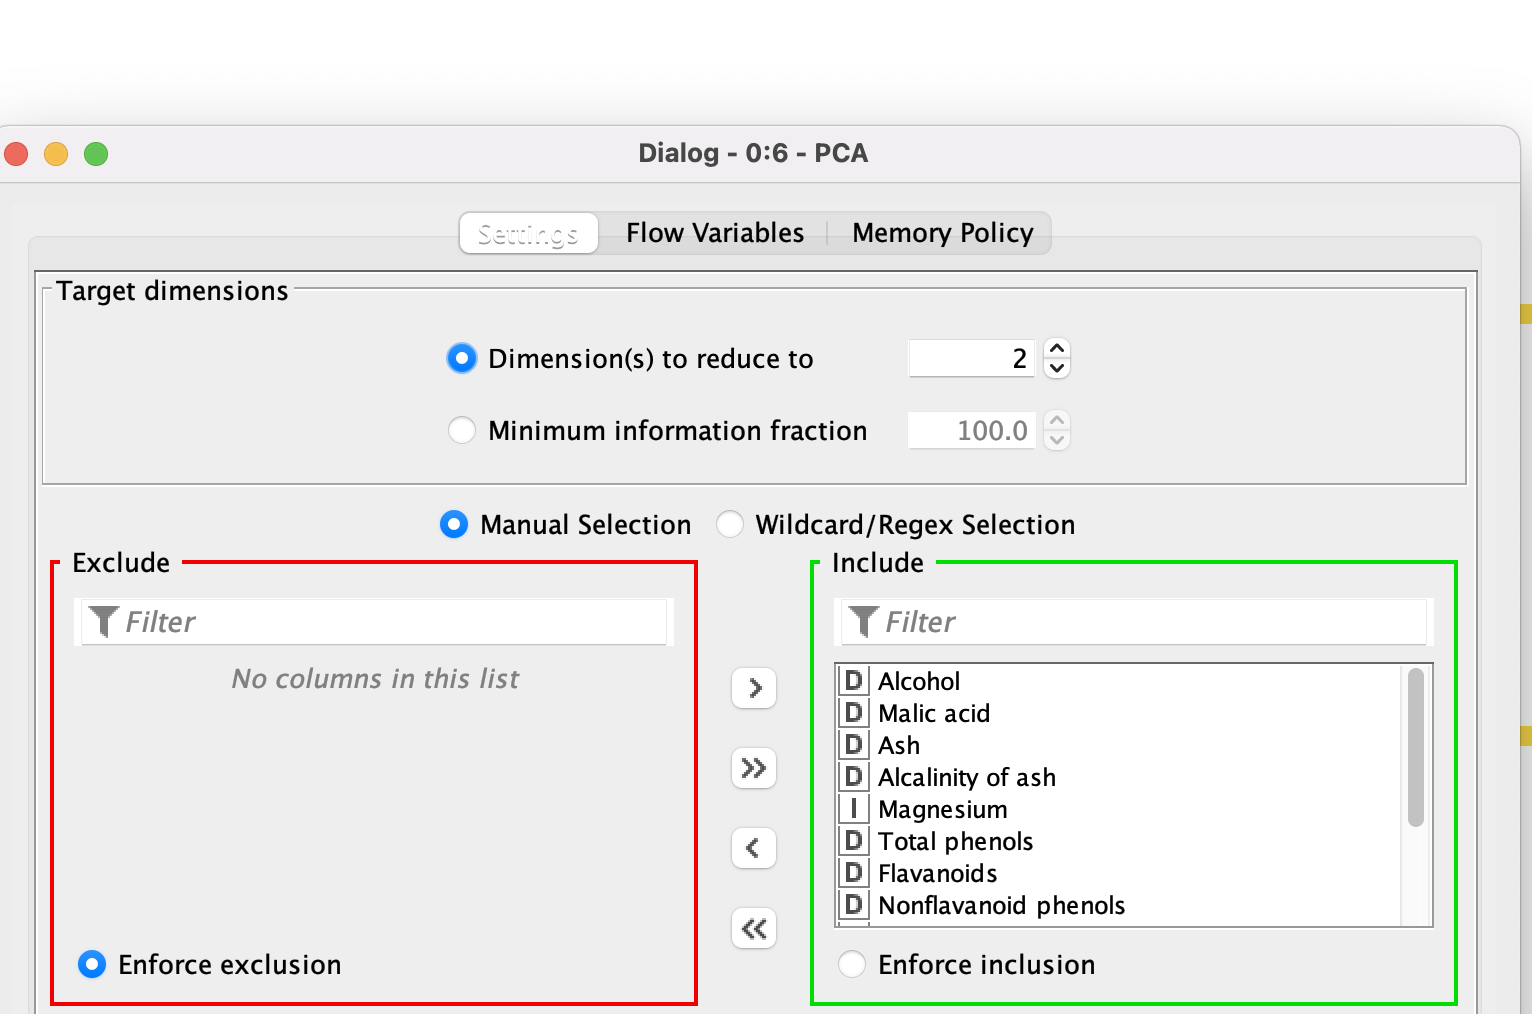
\includegraphics[width=\textwidth]{res/t1/t11/t11-PCA-conf}
					\caption{PCA: The Principal Component Analysis node, we request to reduce the dimensionality to 2, worth mentioning that, as 'class' is a string column, it is automatically excluded from PCA possible columns.}
					\label{fig:first}
				\end{subfigure}
				\hfill
				\begin{subfigure}{0.4\textwidth}
					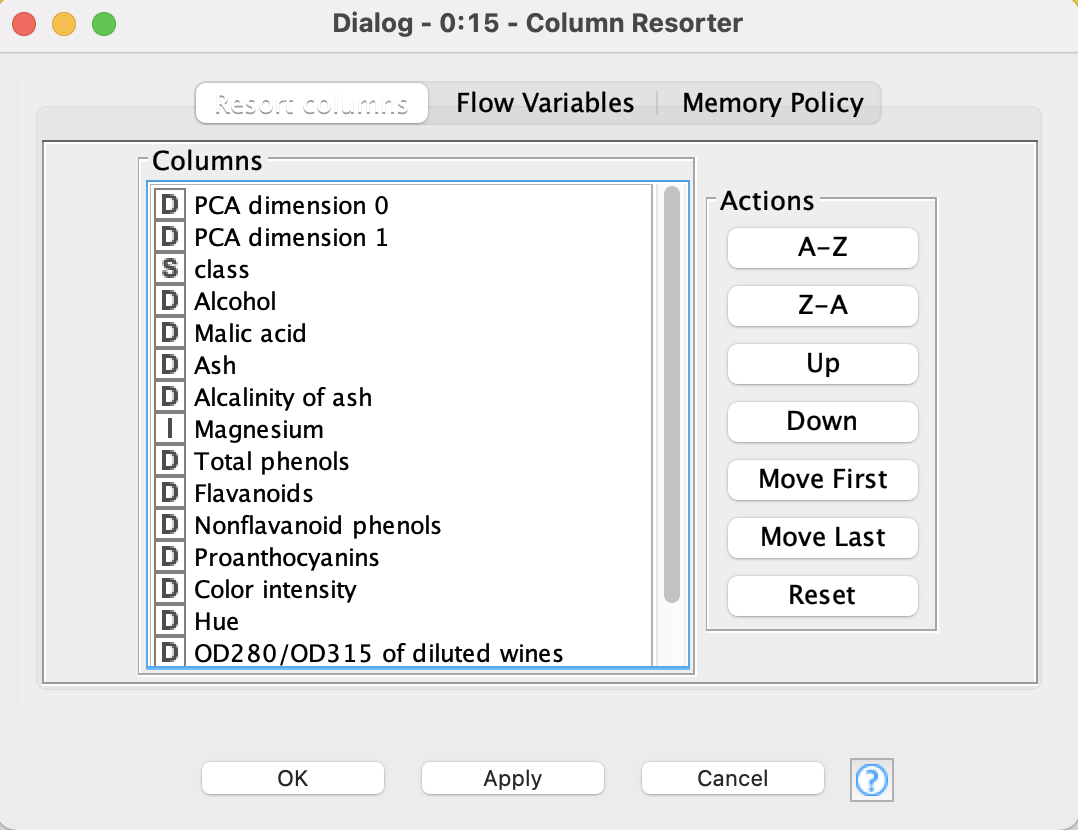
\includegraphics[width=\textwidth]{res/t1/t11/t11-column-resorter-conf}
					\caption{Column Resorter: move first and second principal components on top(first two columns), to be displayed by Scatter Plot Node.}
					\label{fig:second}
				\end{subfigure}
				\hfill
			\end{figure}
			\fi
			Finally, plot1 is given below.
			\iftrue
			\begin{center}
				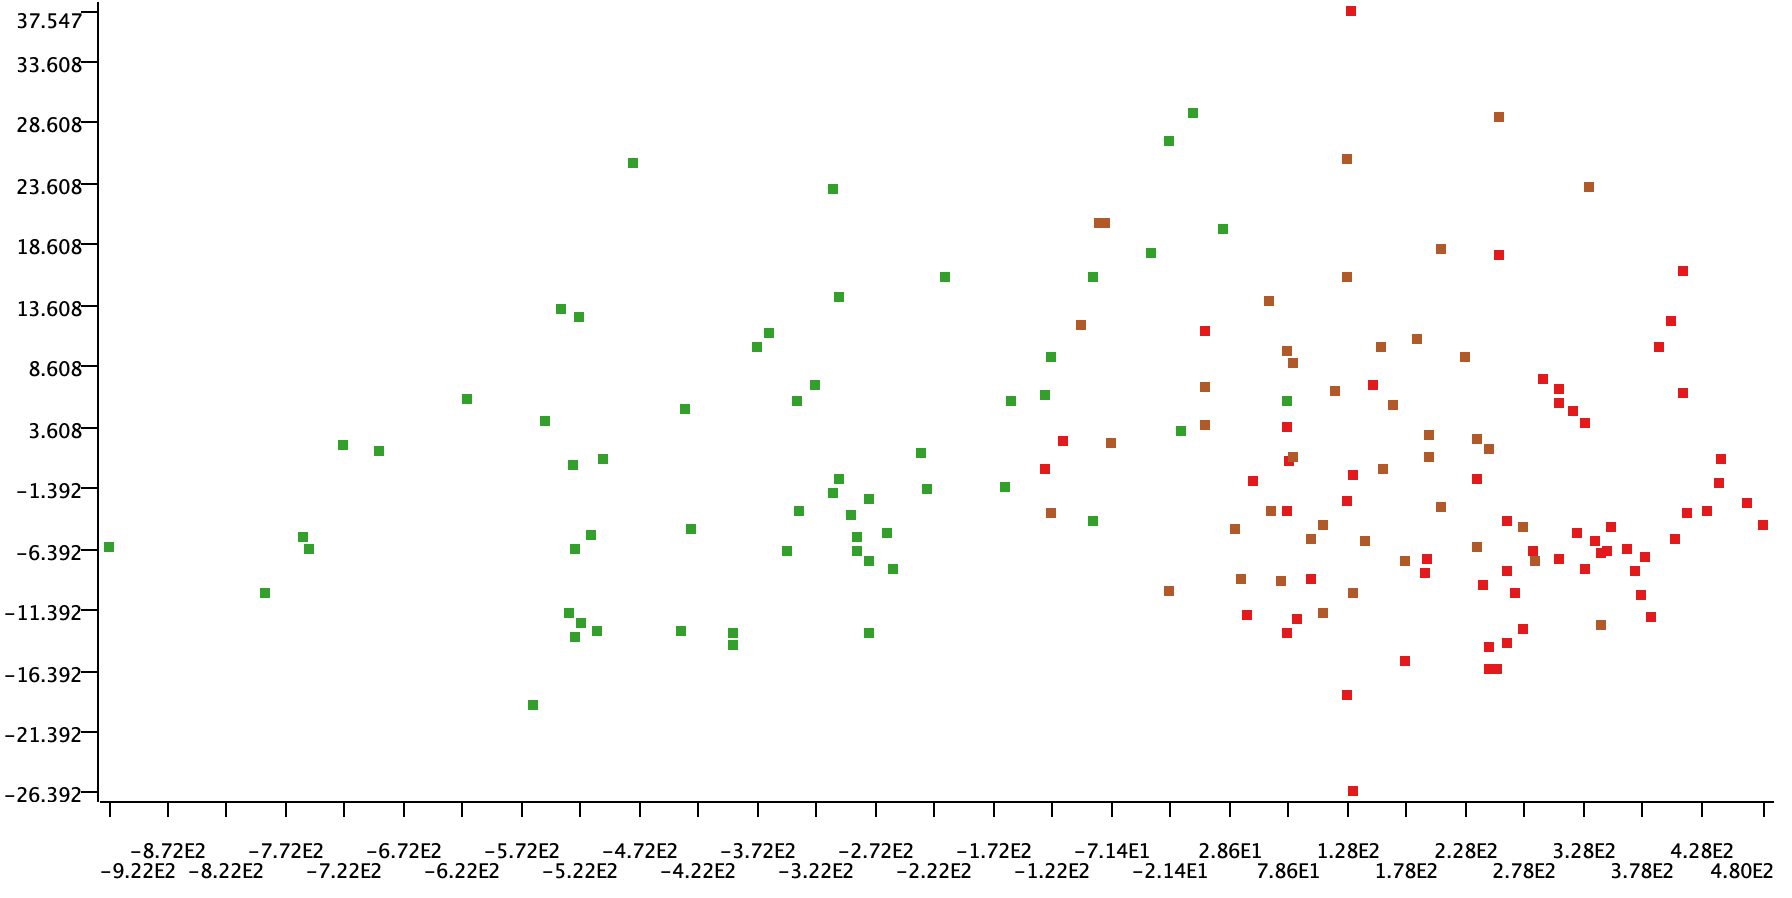
\includegraphics[scale=0.5]{res/t1/t11/t11-plot1}
			\end{center}
			\fi
		\subsection*{Task 1.2 : Generate plot2}
			The workflow to generate plot2 is given below.
			\iftrue
			\begin{center}
				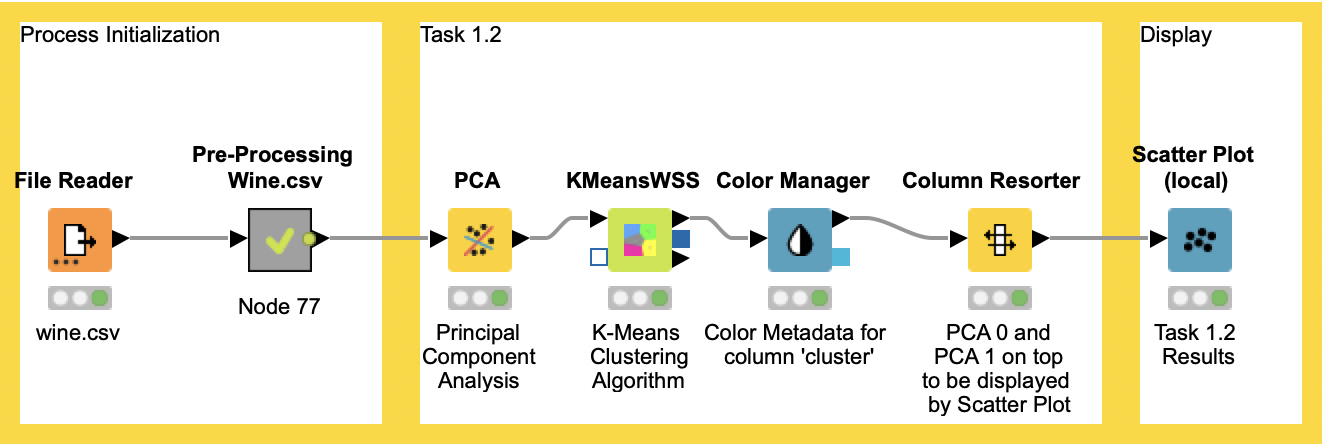
\includegraphics[scale=0.35]{res/t1/t12/t12-workflow}
			\end{center}
			\fi
			Apart from the clustering algorithm adopted(K-Means), there are no significant changes with the workflow from the previous task; please see task1.1 for an overall workflow review. The Newly introduced nodes configurations, as well as the descriptions, are given below.
			
			\iftrue
			\begin{figure}[H]
				\centering
				\begin{subfigure}{0.4\textwidth}
					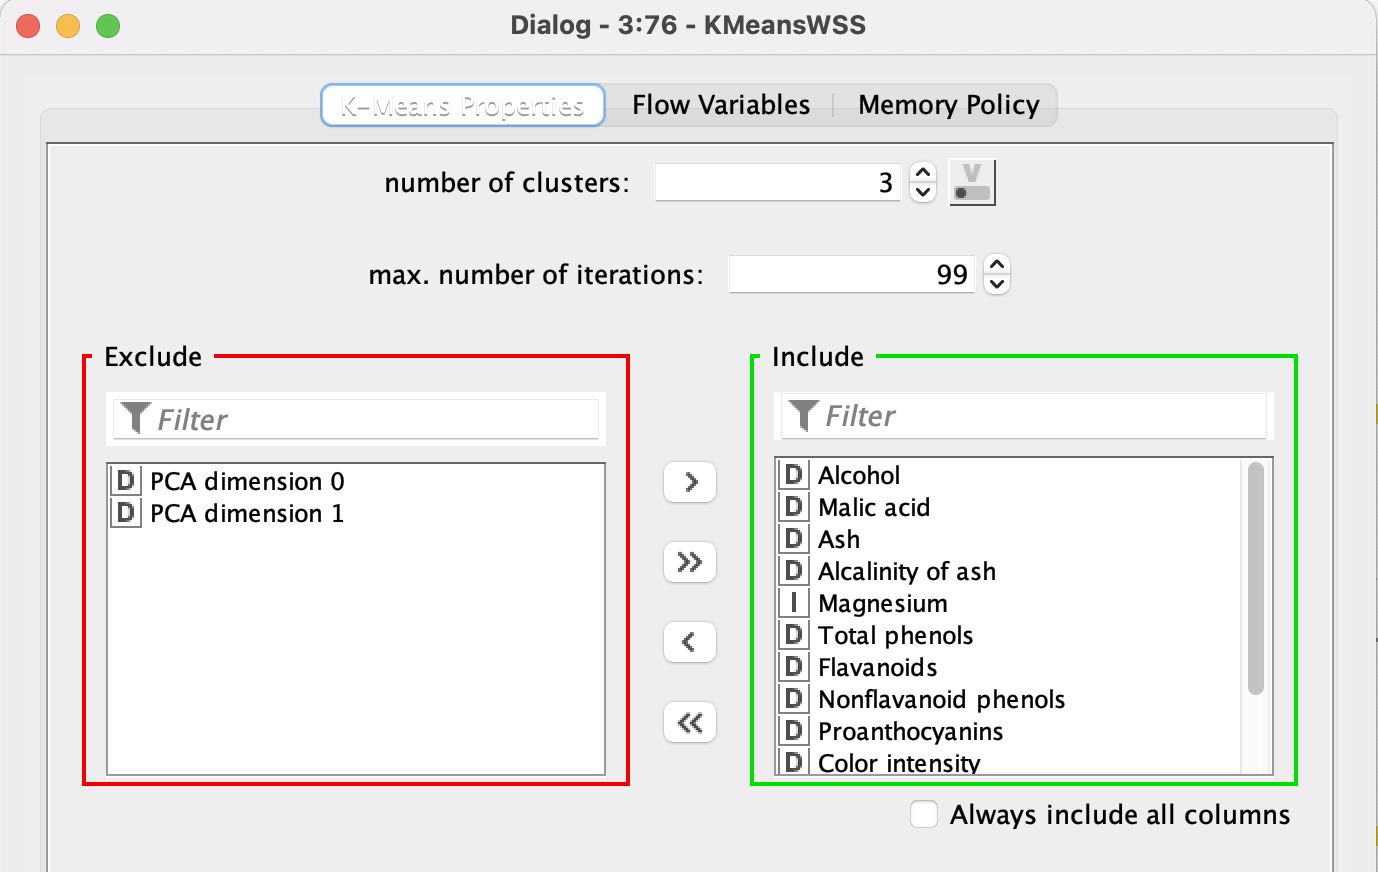
\includegraphics[width=\textwidth]{res/t1/t12/t12-kmeans-wss-conf}
					\caption{KMeansWSS: this node implements our clustering algorithm of choice, the exact inner-workings to be explained in the next paragraph. A noteworthy configuration is the exclusion of PCA dimensions from the clustering process.}
					\label{fig:first}
				\end{subfigure}
				\hfill
				\begin{subfigure}{0.4\textwidth}
					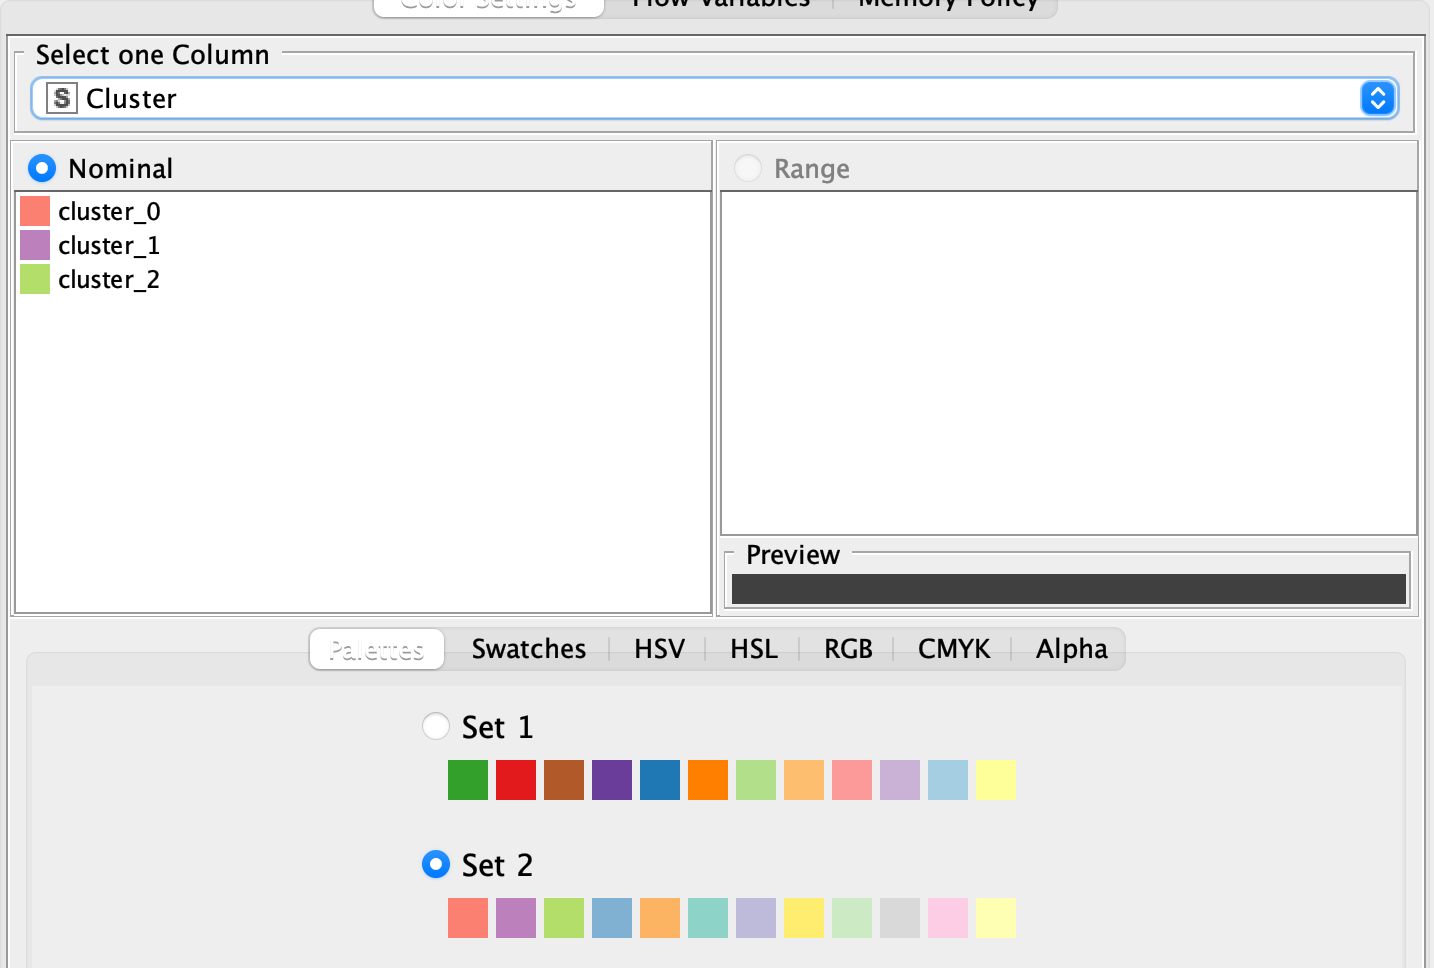
\includegraphics[width=\textwidth]{res/t1/t12/t12-color-manager-conf}
					\caption{Colour Manager: After KMeans finishes, we add colour metadata to our 'cluster' column, generated by the 'KMeansWSS' node mentioned above, to be displayed by the Scatter Plot node. The colour palette is different from the colour palette chosen on Task1.1}
					\label{fig:second}
				\end{subfigure}
				\hfill
			\end{figure}
			\fi
			Finally, plot2 is given below.
			\iftrue
			\begin{center}
				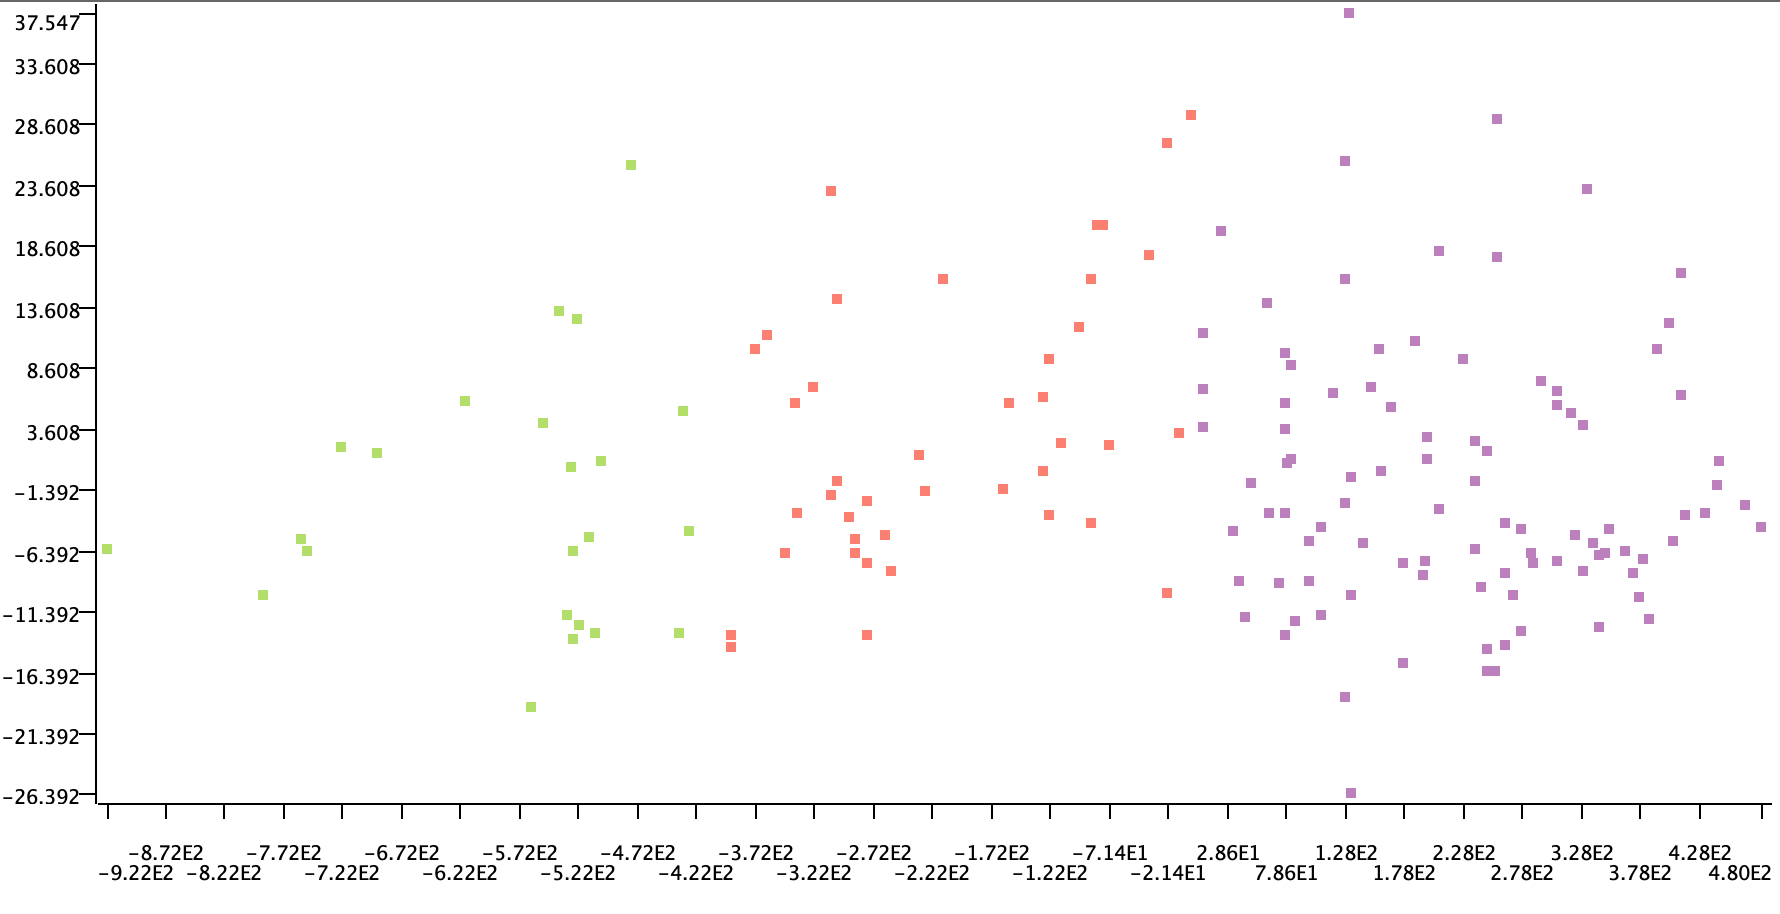
\includegraphics[scale=0.5]{res/t1/t12/t12-plot2}
			\end{center}
			\fi
			\subsubsection*{Introduction to K-Means clustering algorithm}
				K-Means is a heuristic method for grouping {similar} items in clusters. $K$ is the number of clusters and is pre-determined. By heuristic, we mean that the algorithm does not produce absolute optimal solutions but approximations with a given accuracy. By similarity, on purely numeric data, we usually mean a geometric distance metric. Three of the most widely accepted geometric metrics for determining similarity are Euclidean, Manhattan and Minkowski distances.
			\subsubsection*{K-Means Algorithm}
				K-Means is a heuristic algorithm that repeats two distinct steps to converge into an acceptable solution. We will explain K-Means with a hands-on example. Let the following fictional 1D Data, $k=3$.
				\iftrue
				\begin{center}
					
\includegraphics[scale=0.5]{res/t1/t12/t12-kmeans-1}
				\end{center}
				\fi
				Let initialize $k=3$ initial random estimated cluster centroids.
				\iftrue
				\begin{center}
					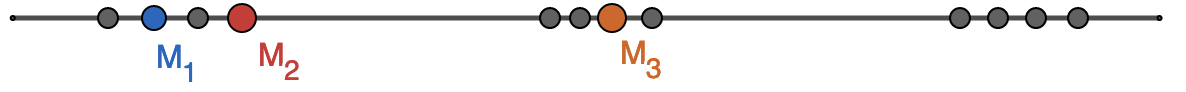
\includegraphics[scale=0.5]{res/t1/t12/t12-kmeans-2}
				\end{center}
				\fi
				Now, the repetitive process, First, we should calculate the distances of any given point from each of the $k=3$ currently estimated cluster centroids. Then, we should assign the given datapoint into the cluster with the closest centroid. Here $X_1$ will be assigned on the blue cluster($M_1$).
				\iftrue
				\begin{center}
					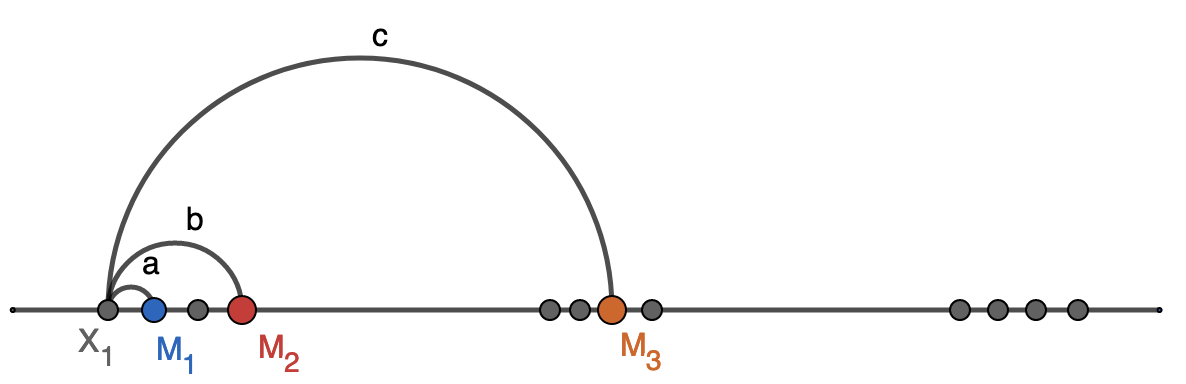
\includegraphics[scale=0.5]{res/t1/t12/t12-kmeans-3}
				\end{center}
				\fi
				After the calculation is finished for all the data points, the clustering should look like the following figure.
				\iftrue
				\begin{center}
					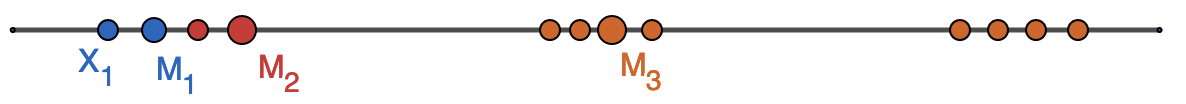
\includegraphics[scale=0.5]{res/t1/t12/t12-kmeans-4}
				\end{center}
				\fi
				We now calculate the centroids of the clusters. The centroids do not need to be actual data points; they can lie anywhere on the domain space.
				\iftrue
				\begin{center}
					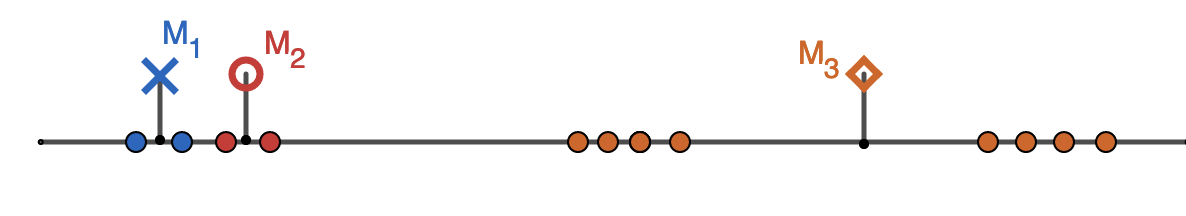
\includegraphics[scale=0.5]{res/t1/t12/t12-kmeans-5}
				\end{center}
				\fi
				We repeat steps 2 and 3 until we end up with an acceptable solution.
				\iftrue
				\begin{center}
					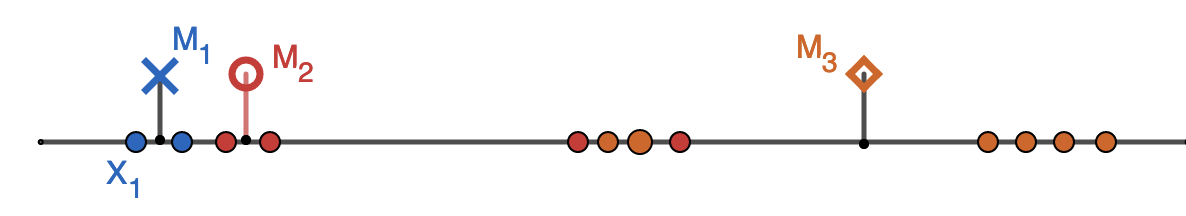
\includegraphics[scale=0.5]{res/t1/t12/t12-kmeans-6}
					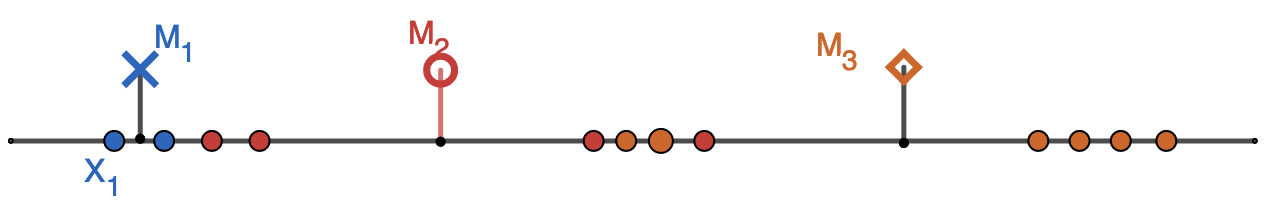
\includegraphics[scale=0.5]{res/t1/t12/t12-kmeans-7}
					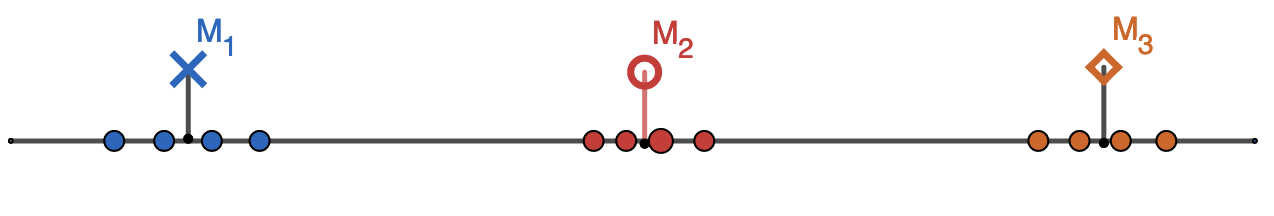
\includegraphics[scale=0.5]{res/t1/t12/t12-kmeans-8}
				\end{center}
				\fi
				We can quantify the quality of a solution(i.e. quantify if the given solution is acceptable) by using the Sum of Squared errors statistic(SSE). K-Means terminates when SSE converges into a value. SEE will be explained in detail on Task 1.5.
				
		 \subsection*{Task 1.3 : Compare plot1 and plot2}
			The main point of interest in the figures above is the fact that the clustering algorithm(K-Means, k=3) failed to appropriately partition the data and recognize the classes provided by the dataset. This phenomenon can be explained due to the absence of the normalization process, something that will be explained in the next task. The exact scale of the problem cannot be appropriately assessed with only those two plots, though we will need to examine the distribution of the classes in each cluster, something that will be done on the next task (Task 1.4).
		
		 \subsection*{Task 1.4 : plot3a,plot3b,plot3c}
			The workflow to generate the requested plots is given below.
			\iftrue
			\begin{center}
				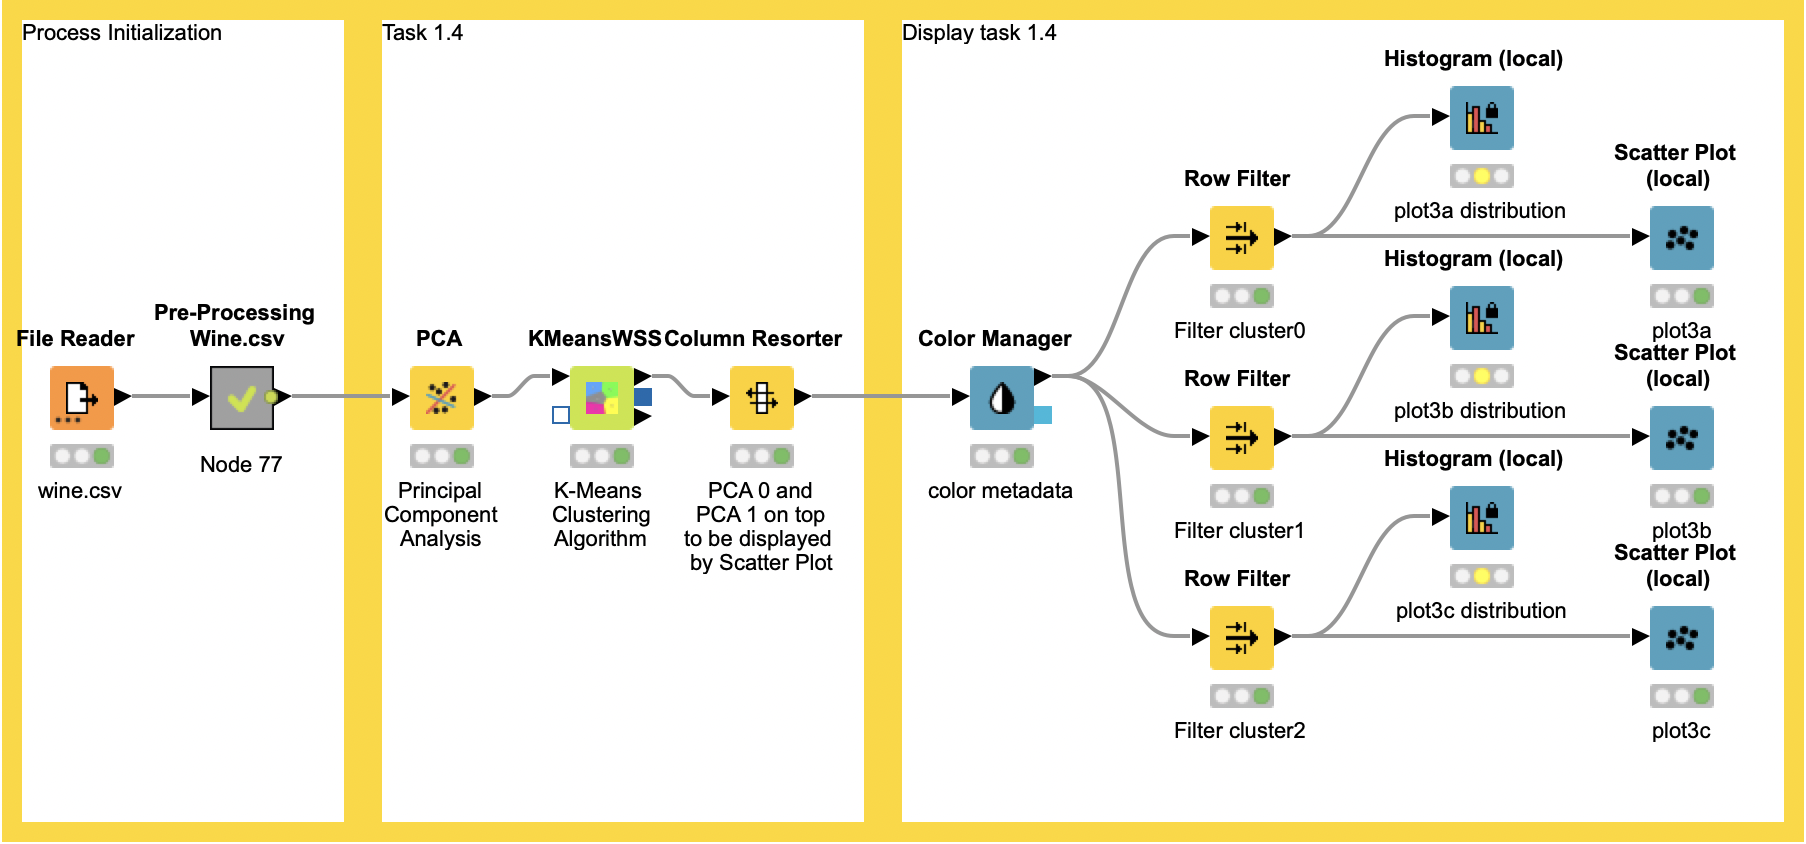
\includegraphics[scale=0.25]{res/t1/t14/t14-workflow}
			\end{center}
			\fi
			The majority of the workflow is identical to task1.1 and task1.2, so please refer to those tasks for detailed explanations of those nodes. The major difference is in the display section. There, we use 3 row filter nodes(one per cluster) to filter the assigned data points on each cluster. Hence in the first plot, we have all the data points assigned to cluster0 and vice versa. The node configurations with the necessary filters are given below.
			\iftrue
			\begin{figure}[H]
				\centering
				\begin{subfigure}{0.4\textwidth}
					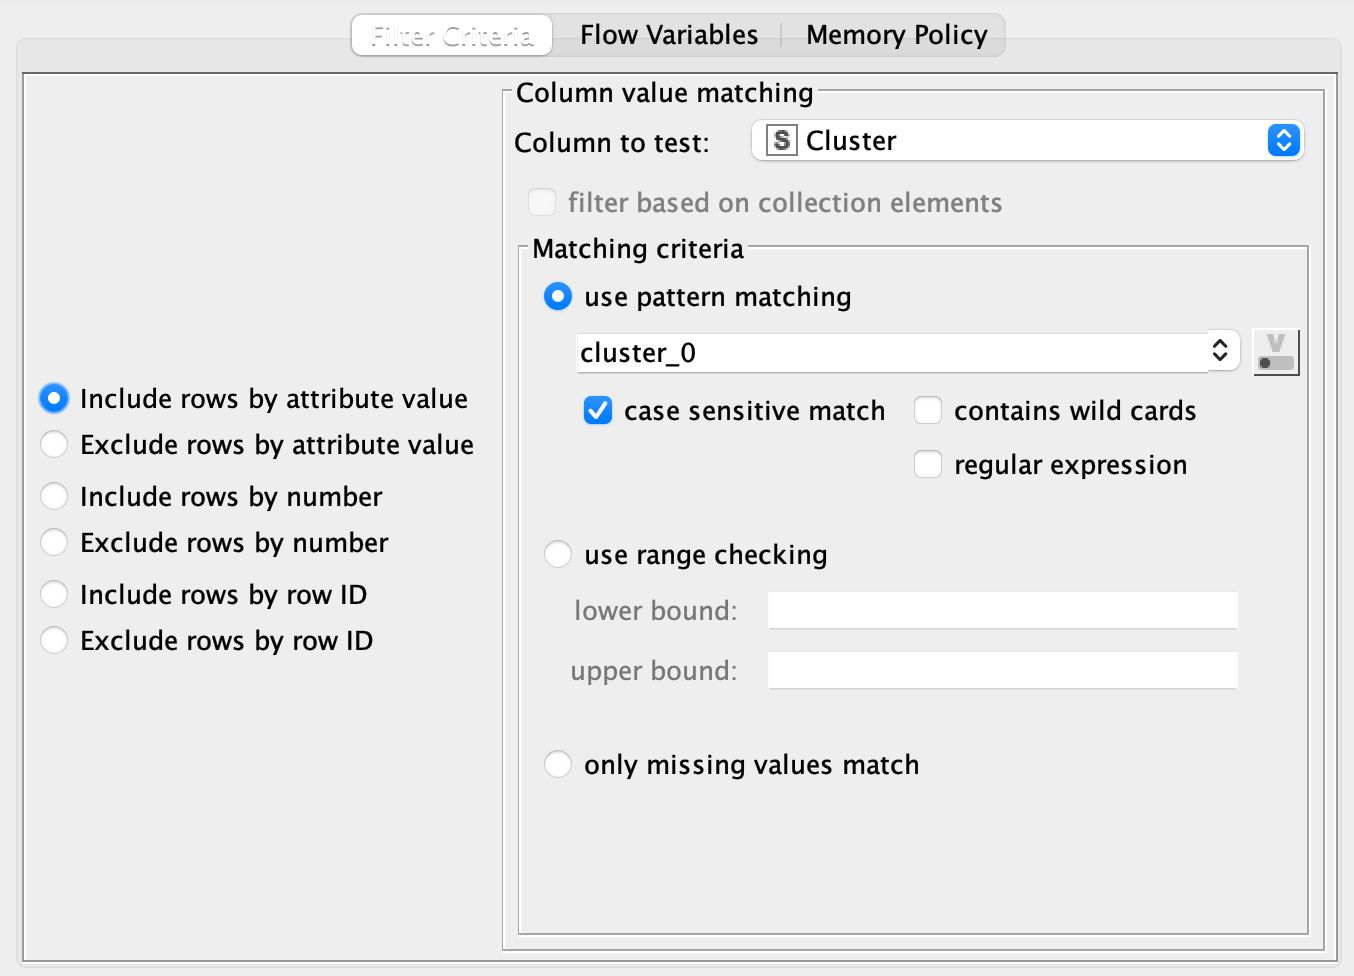
\includegraphics[width=\textwidth]{res/t1/t14/t14-row-filter-1-conf}
					\caption{Row filter: filter datapoint belonging to the first cluster.}
					\label{fig:first}
				\end{subfigure}
				\hfill
				\begin{subfigure}{0.4\textwidth}
					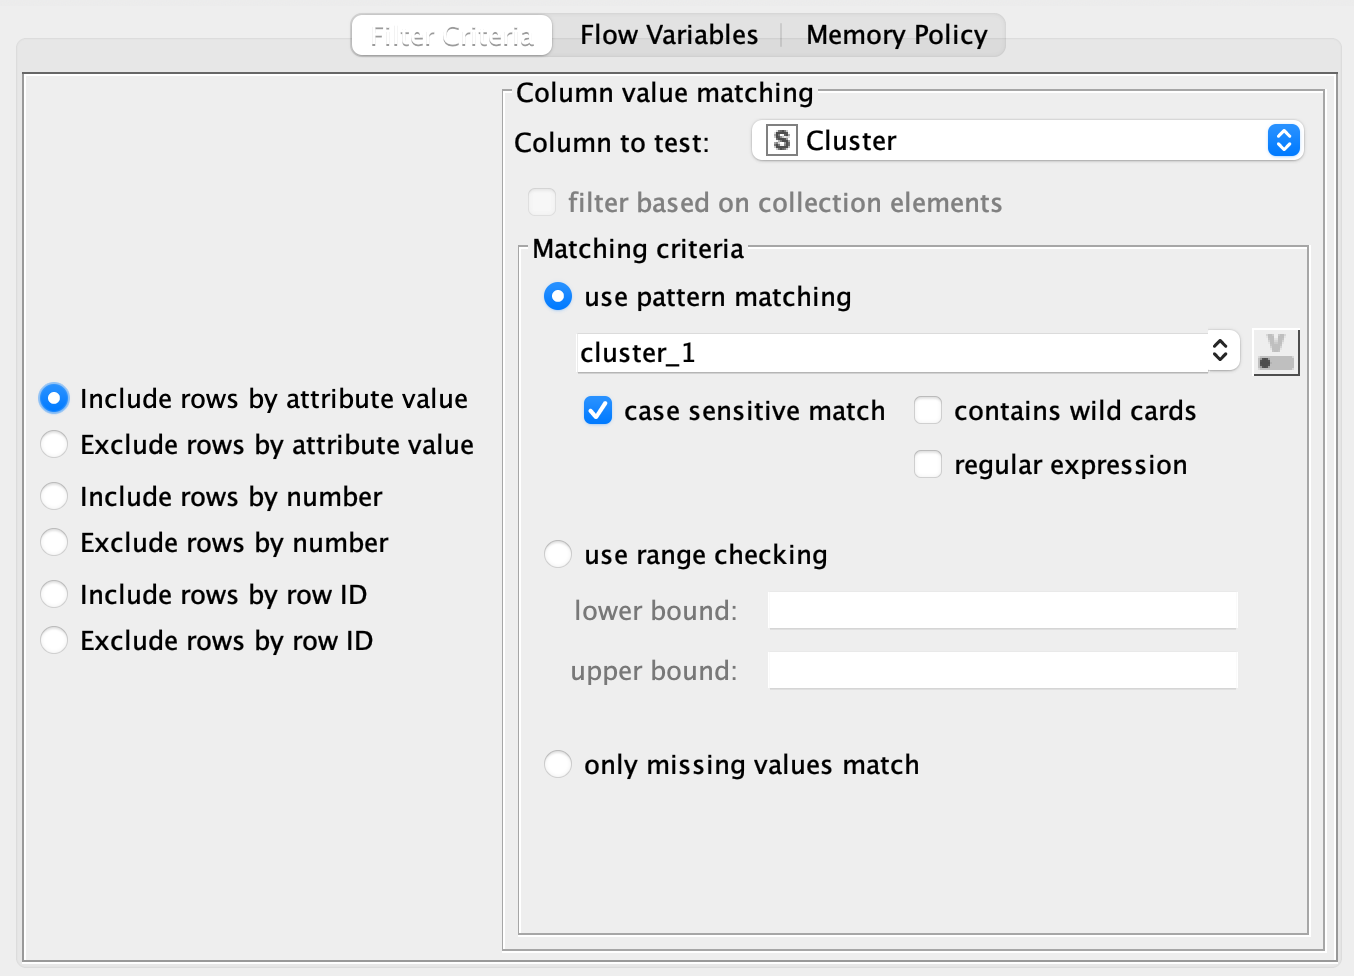
\includegraphics[width=\textwidth]{res/t1/t14/t14-row-filter-2-conf}
					\caption{Row filter: filter datapoint belonging to the second cluster}
					\label{fig:second}
				\end{subfigure}
				\hfill
				\begin{subfigure}{0.4\textwidth}
					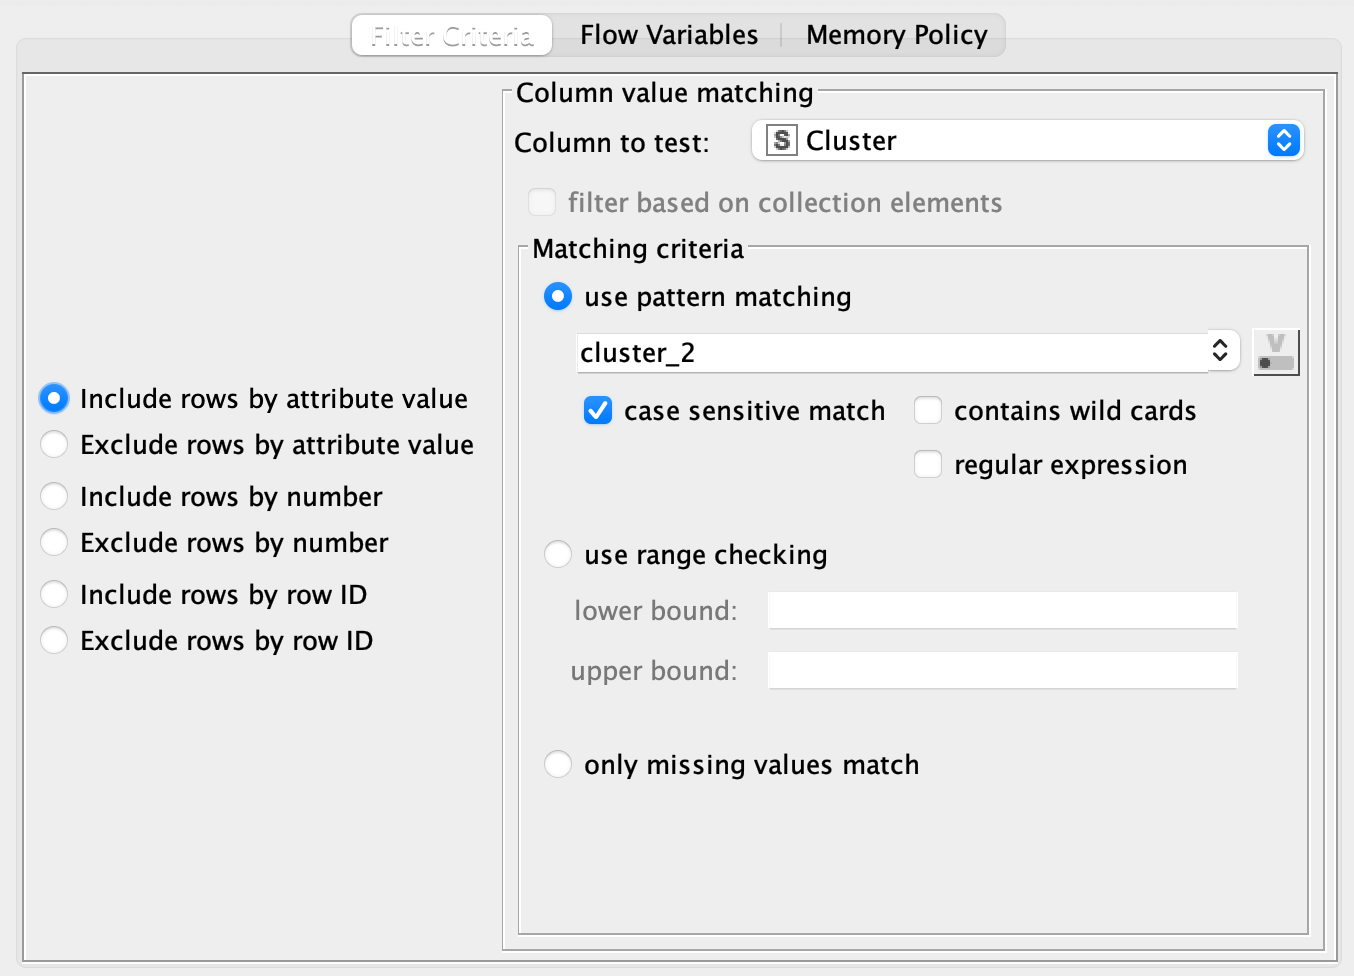
\includegraphics[width=\textwidth]{res/t1/t14/t14-row-filter-3-conf}
					\caption{Row filter: filter datapoint belonging to the third cluster}
					\label{fig:third}
				\end{subfigure}	
				\label{fig:figures}
			\end{figure}
			\fi
			Finally, the generated plots are given in the next figure.
			\iftrue
			 \begin{figure}[H]
			 	\centering
			 	\begin{subfigure}{0.4\textwidth}
			 		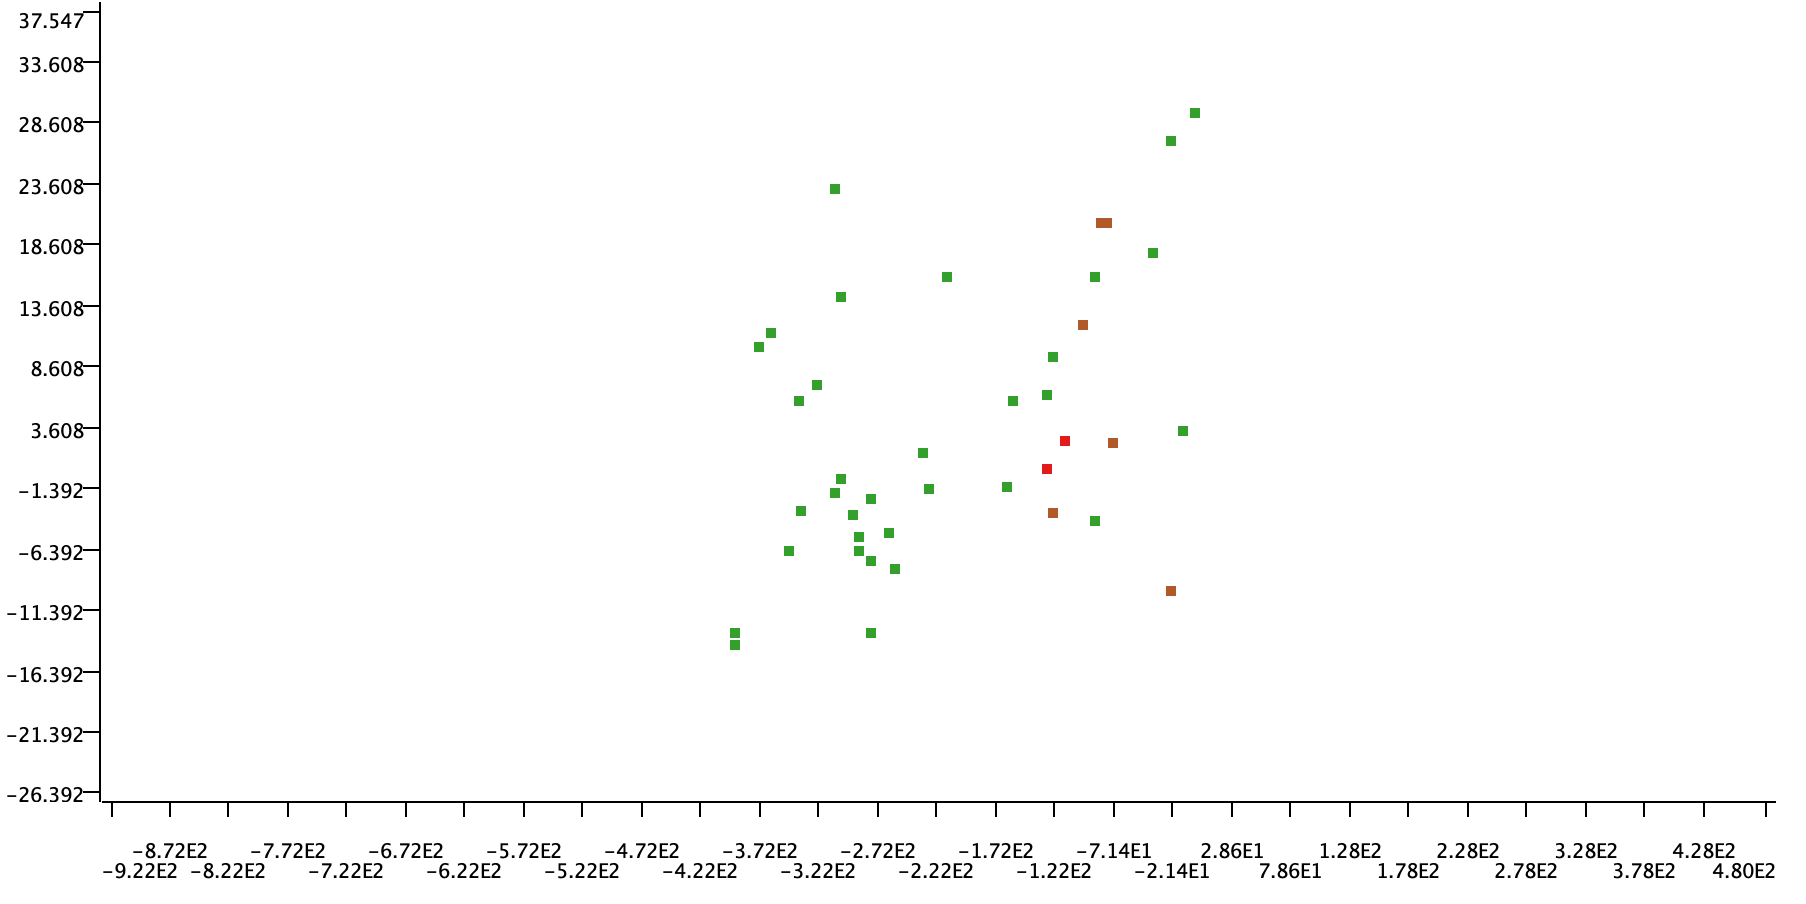
\includegraphics[width=\textwidth]{res/t1/t14/t14-plot3a}
			 		\caption{plot3a}
			 		\label{fig:first}
			 	\end{subfigure}
			 	\hfill
			 	\begin{subfigure}{0.4\textwidth}
			 		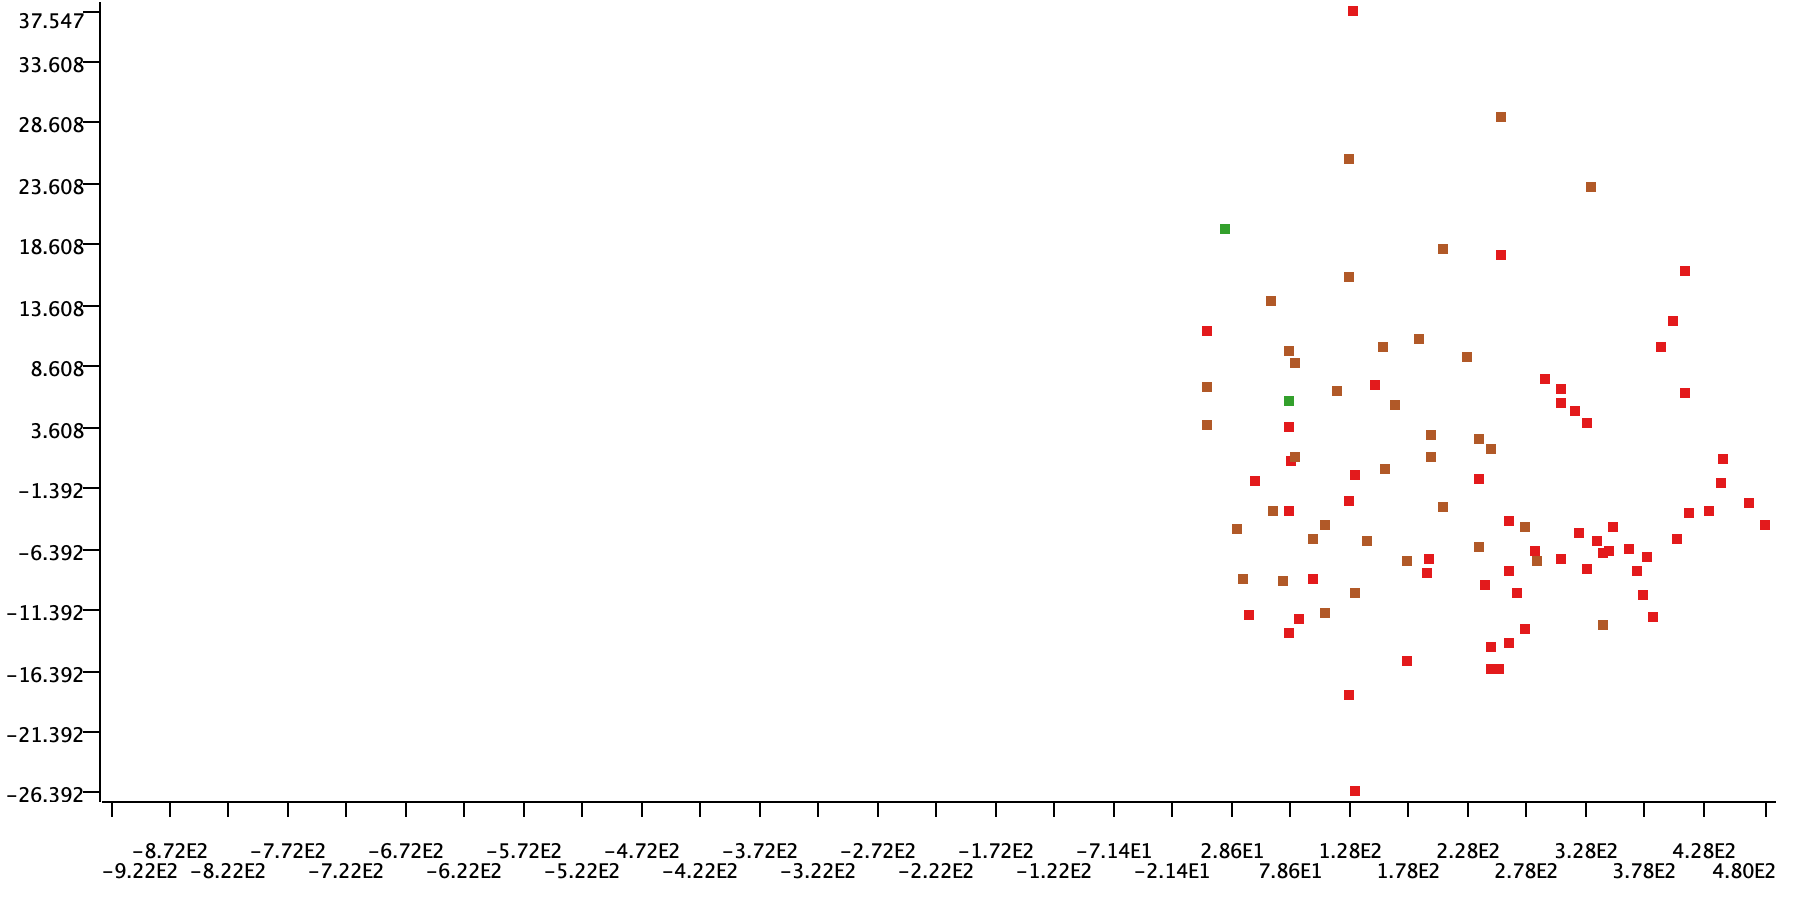
\includegraphics[width=\textwidth]{res/t1/t14/t14-plot3b}
			 		\caption{plot3b}
			 		\label{fig:second}
			 	\end{subfigure}
			 	\hfill
			 	\begin{subfigure}{0.4\textwidth}
			 		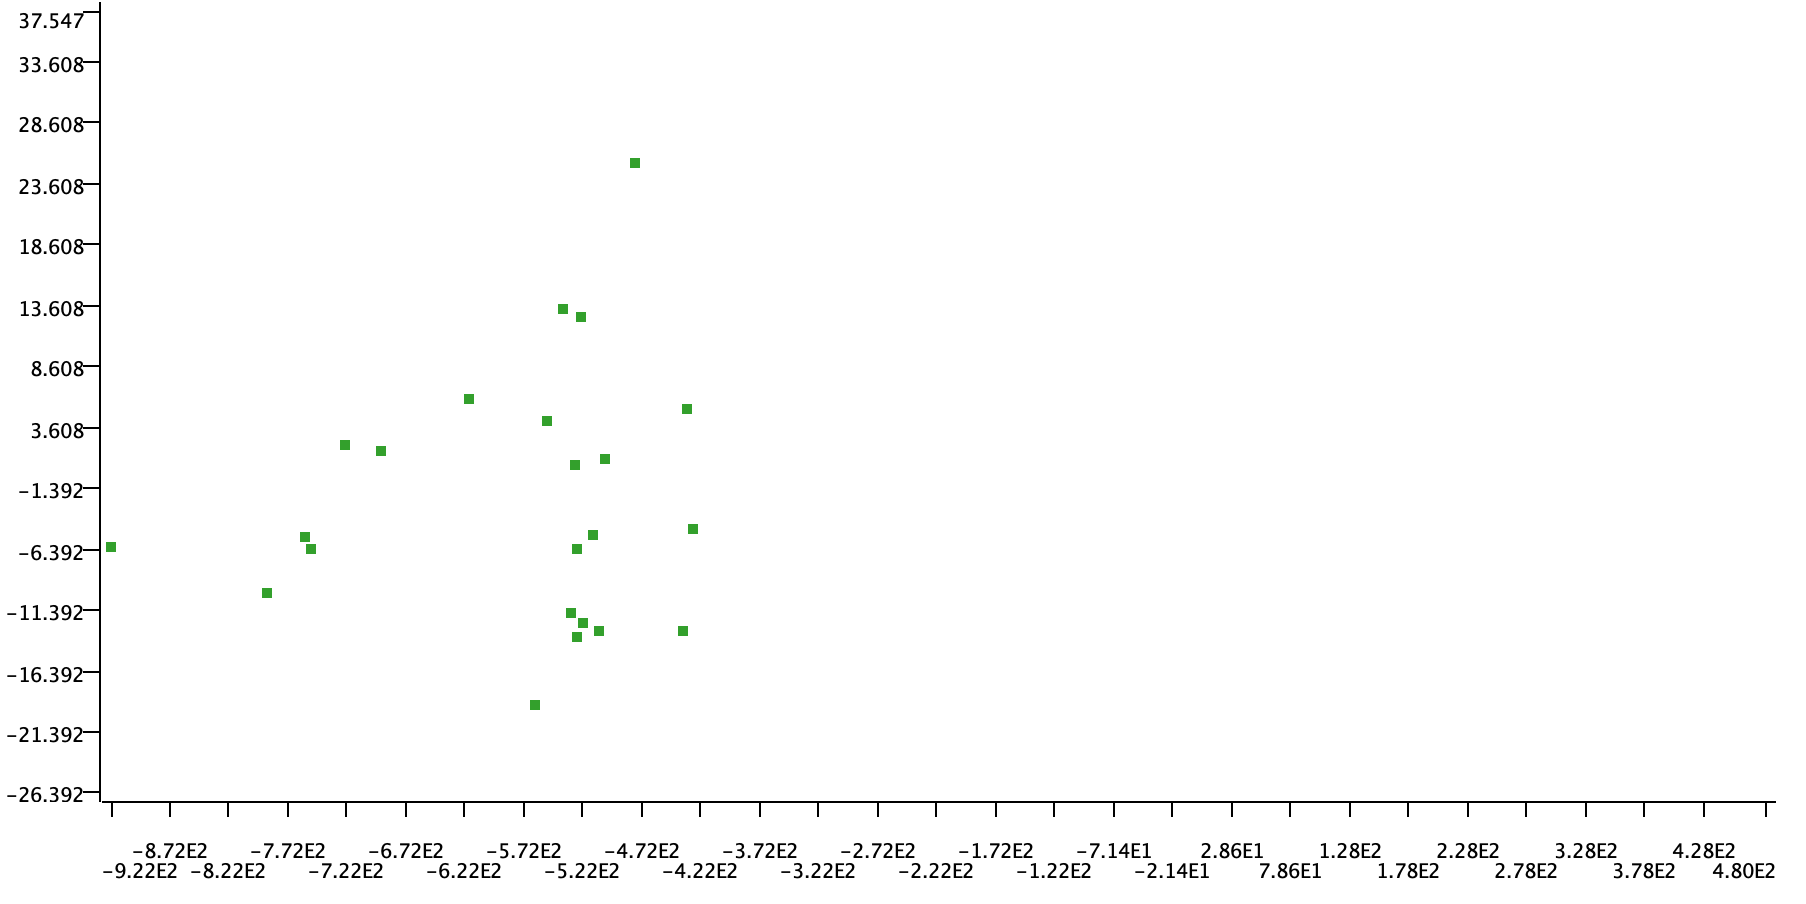
\includegraphics[width=\textwidth]{res/t1/t14/t14-plot3c}
			 		\caption{plot3c}
			 		\label{fig:third}
			 	\end{subfigure}
			 	\label{fig:figures} 
			 \end{figure}
		 	\fi
			It becomes apparent that the clusters generated compose a meaningless clustering solution. Under ideal circumstances, each cluster will have a vast majority of each of the classes, with some to no variation due to outliers or errors; using histograms, we can visualize the extent of the issue 
			\iftrue
			\begin{figure}[H]
				\centering
				\begin{subfigure}{0.4\textwidth}
			 		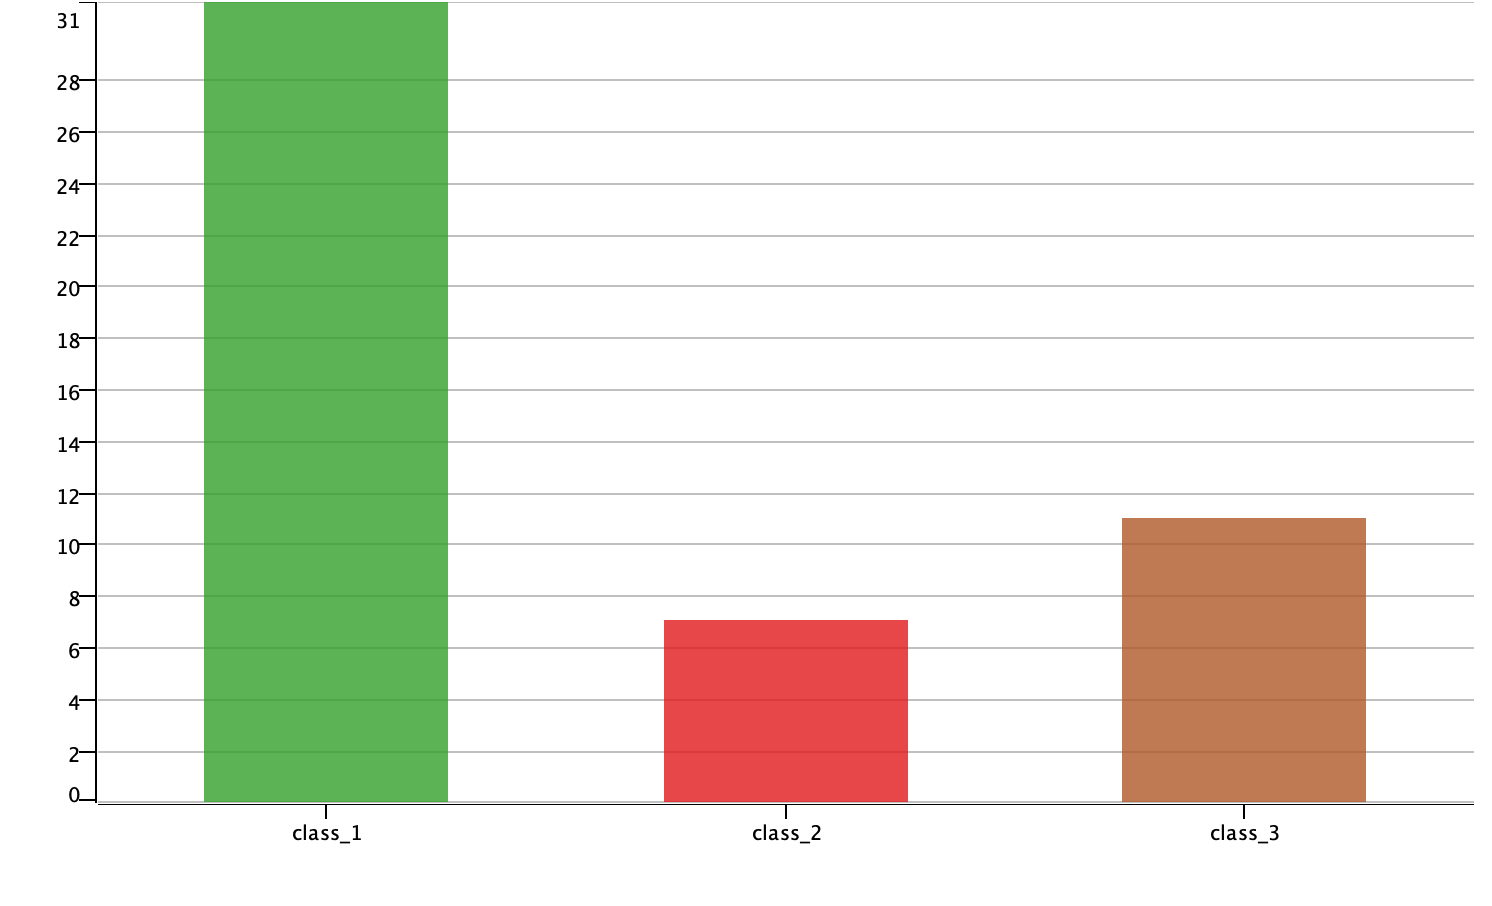
\includegraphics[width=\textwidth]{res/t1/t14/t14-plota-dist}
					\caption{plot3a distribution}
					\label{fig:first}
				\end{subfigure}
				\hfill
				\begin{subfigure}{0.4\textwidth}
			 		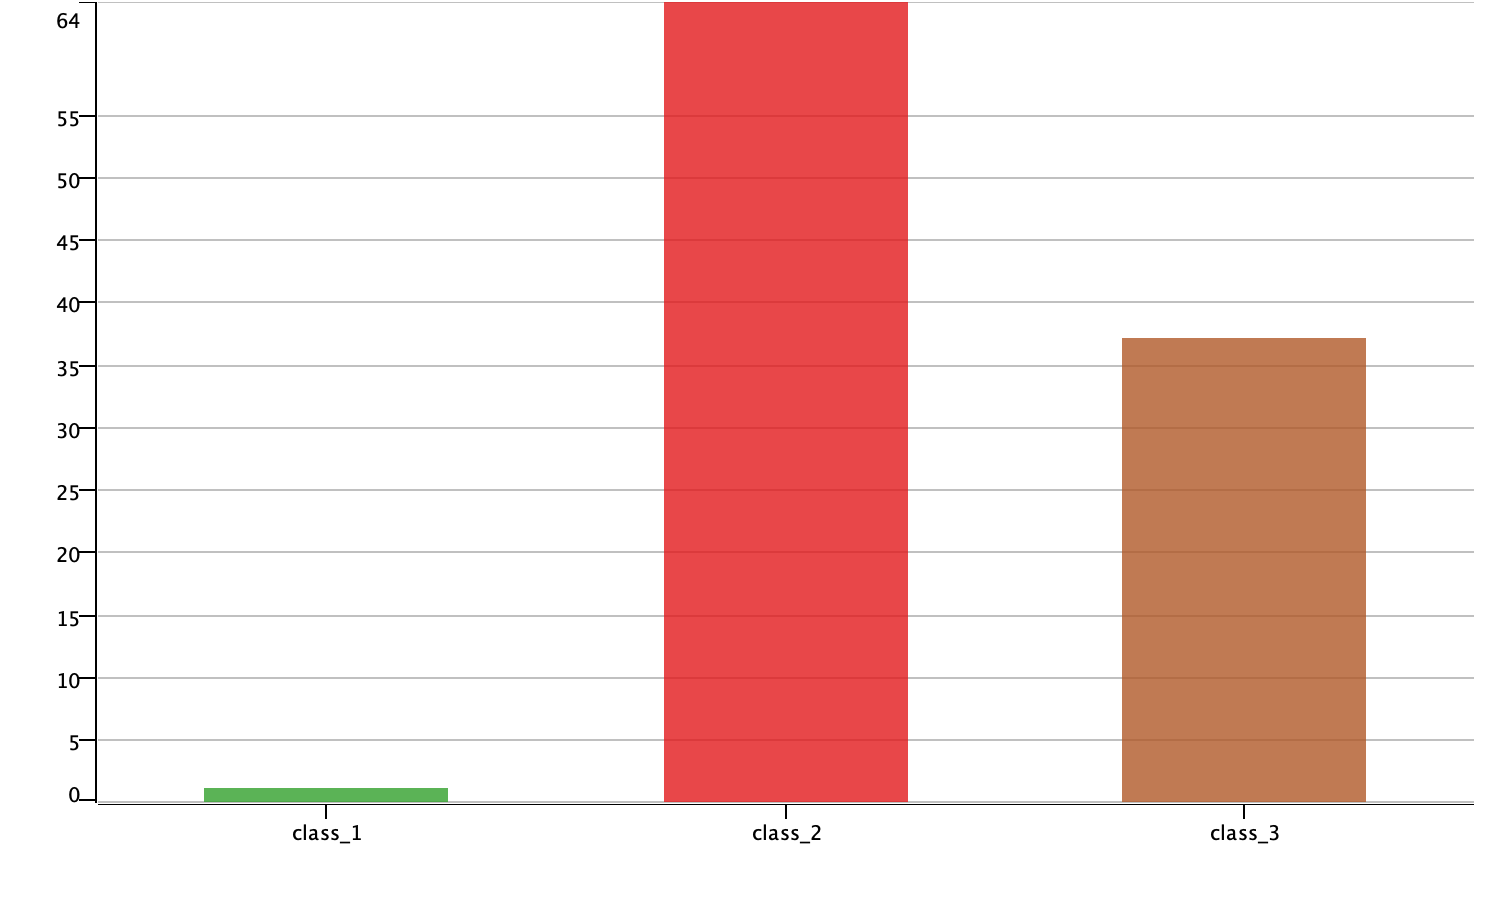
\includegraphics[width=\textwidth]{res/t1/t14/t14-plotb-dist}
					\caption{plot3b distribution}
					\label{fig:second}
				\end{subfigure}
				\hfill
				\begin{subfigure}{0.4\textwidth}
			 		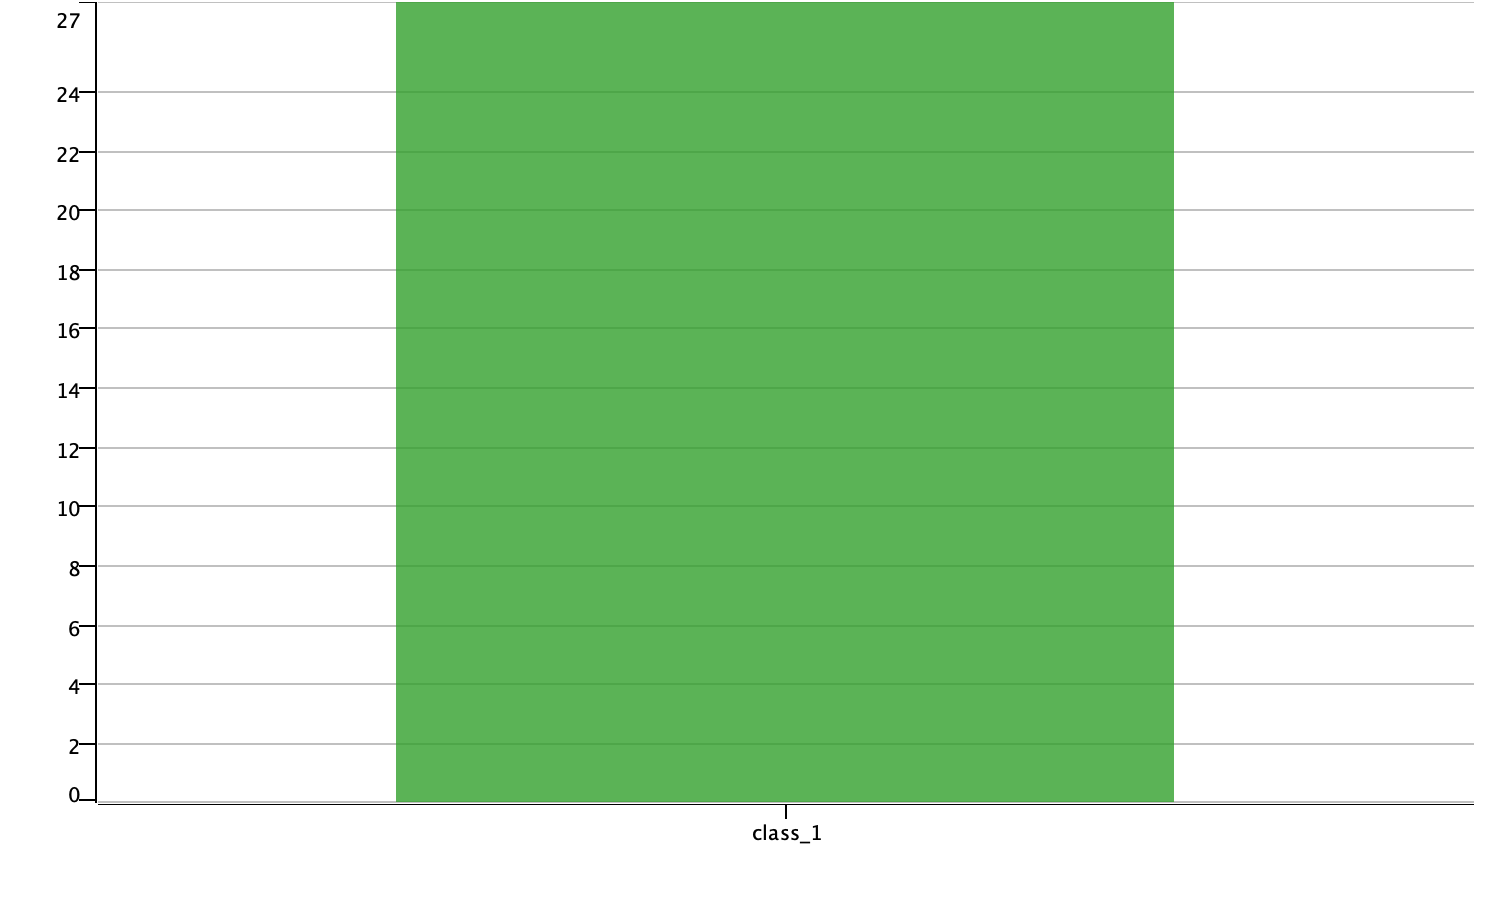
\includegraphics[width=\textwidth]{res/t1/t14/t14-plotc-dist}
					\caption{plot3c distribution}
					\label{fig:third}
				\end{subfigure}	
				\label{fig:figures}
			\end{figure}
			\fi
			 This is the result of the lack of a normalization process, something that we will explain on the next task.
		\subsection*{Task 1.5 : Cluster Validity Measure}
			For our cluster validity measure, we will explain and interpret WSS (Within cluster sum of squares) and BSS (Between cluster sum of squares). The workflow for generating the cluster validity measures is given below.
			\iftrue
			\begin{center}
				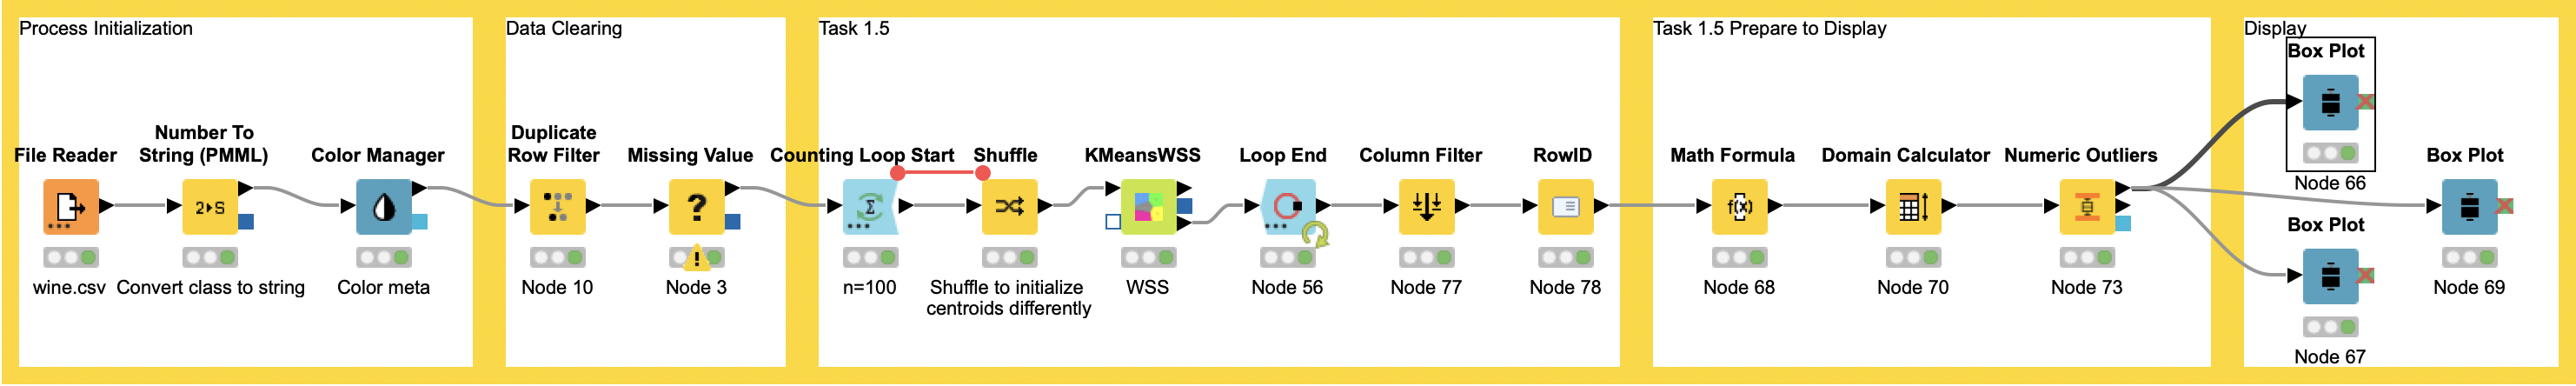
\includegraphics[scale=0.25]{res/t1/t15/t15-workflow}
			\end{center}
			\fi
			The majority of the workflow is identical to workflows of task1.1 to task1.4, so please refer to those tasks for a detailed explanations of those nodes. The Major Difference is on the repeat process and on the intepretation proccess. The newrly introduced nodes configurations are given below, along with a short explanation
			\iftrue
			\begin{figure}[H]
				\centering
				\begin{subfigure}{0.35\textwidth}
					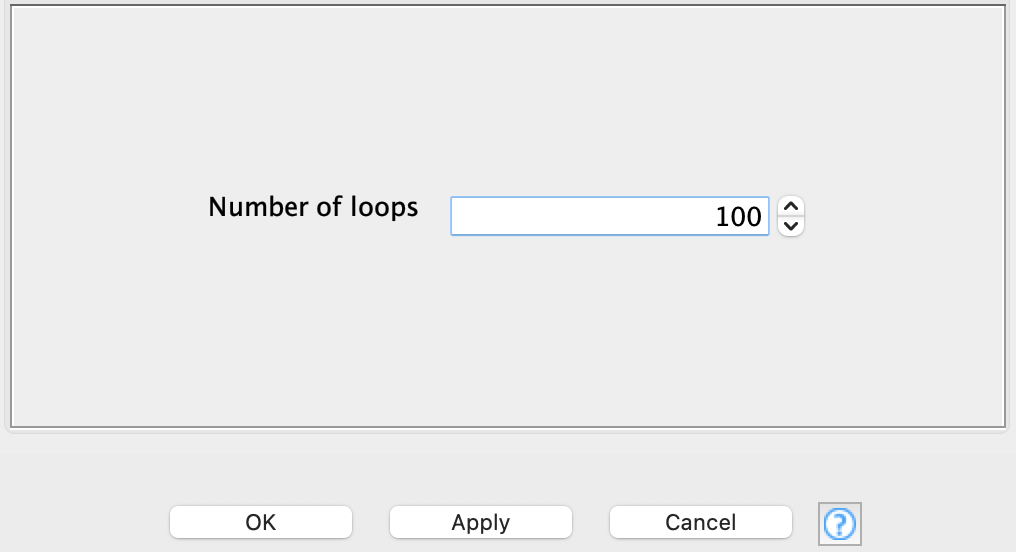
\includegraphics[width=\textwidth]{res/t1/t15/t15-counting-loop-start-conf}
					\caption{Counting Loop Start: Because of K-Means is a heuristic algorithm; it makes sense to be analysed in a series of runs, we will run for $n=100$. That's necessary because of the fact that every heuristic algorithm is vulnerable to being stuck onto a local-minima and producing biased/wrong results\cite{local-minima}.}
					\label{fig:first}
				\end{subfigure}
				\hfill
				\begin{subfigure}{0.35\textwidth}
					\includegraphics[width=\textwidth]{res/t1/t15/t15-shuffle-conf}
					\caption{Shuffle: This K-Means implementation gets initialized by setting the first k elements as centroids. In order to evaluate the behaviour of the algorithm, we need to shuffle our dataset to enforce K-Means to initialise with different centroids. \cite{k-means-init}}
					\label{fig:second}
				\end{subfigure}
				\hfill
				\begin{subfigure}{0.35\textwidth}
					\includegraphics[width=\textwidth]{res/t1/t15/t15-loop-end-conf}
					\caption{Loop End: The only noteworthy mention here is the fact that we append a new column containing the number of iteration.}
					\label{fig:third}
				\end{subfigure}	
				\begin{subfigure}{0.4\textwidth}
					\includegraphics[width=\textwidth]{res/t1/t15/t15-row-id-conf}
					\caption{Row ID: Use the number of iterations as RowID column}
					\label{fig:first}
				\end{subfigure}
				\hfill
				\begin{subfigure}{0.35\textwidth}
					\includegraphics[width=\textwidth]{res/t1/t15/t15-math-formula-conf}
					\caption{Math Formula: A nice way to visualize the performance of K-Means, is to calculate the ratio of $\frac{WSS}{BSS}$, more on that on the 'interpretation' part.}
					\label{fig:second}
				\end{subfigure}
				\hfill
				\begin{subfigure}{0.35\textwidth}
					\includegraphics[width=\textwidth]{res/t1/t15/t15-domain-calculator-conf}
					\caption{Domain Calculator: As we involve tiny numbers, we need to explicitly tell KNIME to keep the ranges (not to round) as much as possible.}
					\label{fig:third}
				\end{subfigure}	
				\begin{subfigure}{0.35\textwidth}
					\includegraphics[width=\textwidth]{res/t1/t15/t15-numeric-outliers-conf}
					\caption{Numeric Outliers: To extract insightful box plots, we need to eliminate outliers(very bad initializations).}
					\label{fig:first}
				\end{subfigure}
					\label{fig:figures}
			\end{figure}
			\fi
			
			\subsubsection*{WSS and BSS Explained, Prerequisites}
				Before we attempt explaining WSS and BSS, it is essential to explain SSE (Sum of Square estimate of Errors). SSE is an evaluation metric with a plethora of applications in statistics and predictive analytics\cite{sse}. It is used to evaluate a model's performance against a training set. The logic behind SSE is rather simple. Let X a random variable and a model $y=\bar{X}$.
				\iftrue
				\begin{center}
					\includegraphics[scale=0.5]{res/t1/t15/t15-SSE}				
				\end{center}
				\fi
				We can evaluate our model's performance by calculating the Sum of Errors, where 'error', in this case, is the distance of the observed variable from the response of our model (i.e. the mean $\bar{X}$), as follows
				\iftrue
				\begin{align}
					SE = \sum_{i=1}^{n}{X_i-\bar{X}}
				\end{align}
				\fi
				Unfortunately, our evaluation metric has a fatal flaw; it allows for error's to 'cancel out' simply because they are placed beneath our model's line. It can be proven that for the case of $y=\bar{X}$ SE is always 0.
				\iftrue
				\begin{align}
					SE = \sum_{i=1}^{n}{X_i-\bar{X}} \\
					SE = \sum_{i=1}^{n}{X_i} - \sum_{i=1}{n}{\bar{X}} \\
					SE = \sum_{i=1}^{n}{X_i} - n\bar{X} \\
					SE = \sum_{i=1}^{n}{X_i} - \sum_{i=1}^{n}{X_i} \\
					SE = 0 \\
				\end{align}
				\fi
				For other models(in higher dimensions, where the correlation of the involved variables is not 1), it may not be zero, but the fatal flaw remains; by cancelling errors, we severely underestimate the errors involved. A more appropriate approach could be to square the distances, which would give us the Sum of Squared Errors (SSE).\\
				\iftrue
				\begin{align}
					SSE = \sum_{i=1}^{n}{(X_i-\bar{X})}^2
				\end{align}
				\fi
			\subsubsection*{WSS and BSS Inner-Workings}
				In the world of Clustering models performance evaluation, SSE is translated into two distinct but related ideas, WSS and BSS.
				\iftrue
				\begin{figure}[H]
					\centering
					\begin{subfigure}{0.4\textwidth}
						\includegraphics[width=\textwidth]{res/t1/t15/t15-WSS}
						\caption{WSS}
						\label{fig:first}
					\end{subfigure}
					\hfill
					\begin{subfigure}{0.4\textwidth}
						\includegraphics[width=\textwidth]{res/t1/t15/t15-BSS}
						\caption{BSS}
						\label{fig:second}
					\end{subfigure}
					\hfill
					\label{fig:figures}
				\end{figure}
				\fi
			\subsubsection*{WSS}
				WSS or  Within Cluster Sum of Squares is a clustering model performance evaluation function. Our 'model' in this case is the cluster centroid, and the error is the distance for each data point from the cluster centroid. WSS can be evaluated with the following formula\cite{sse}
				\iftrue
				\begin{align}
					WSS = \sum_{i=1}^{k}{\sum_{x\in{C_i}}^{}{(x-m_i)^2}}	
				\end{align}
				\fi
				Where $k$, the number of clusters involved, $C_i$ the individual cluster and $m_i$, the given cluster centroid.
				\subsubsection*{BSS}
				BSS or  Between Cluster Sum of Squares is a clustering model performance evaluation function, just like WSS. Our 'model' in this case is the overall data mean, and the error is the distance of each cluster's centroid to the overall mean. BSS can be evaluated with the following formula\cite{sse}
				\iftrue
				\begin{align}
					BSS = \sum_{i=1}^{k}{\abs{C_i}(m-m_i)^2}	
				\end{align}
				\fi
				Where $k$, the number of clusters involved, $C_i$ the individual cluster and $m_i$, the given cluster centroid.
			\subsubsection*{Interpretation}
				A good clustering solution would involve well-separated clusters with low WSS to BSS ratio\cite{7}. As K-Means is a heuristic-based algorithm, we will not analyse WSS and BSS of a single K-Means run, but rather we will analyse their behaviour after a sequence of 100 runs. 
				\iftrue
				\begin{figure}[H]
					
					\centering
					\begin{subfigure}{0.4\textwidth}
						\includegraphics[width=\textwidth]{res/t1/t15/t15-WSS-plot}
						\caption{WSS}
						\label{fig:first}
					\end{subfigure}
					\hfill
					\begin{subfigure}{0.4\textwidth}
						\includegraphics[width=\textwidth]{res/t1/t15/t15-BSS-plot}
						\caption{BSS}
						\label{fig:second}
					\end{subfigure}
					\hfill
					\begin{subfigure}{0.4\textwidth}
						\includegraphics[width=\textwidth]{res/t1/t15/t15-Ratio-plot}
						\caption{Ratio}
						\label{fig:third}
					\end{subfigure}
					\label{fig:figures}	
				\end{figure}
				\fi
				It is rather evident that the $\frac{WSS}{BSS}$ Ratio is quite small, something that indicates well-separated clusters(i.e. a good clustering solution). However, a single cluster validity measure is insufficient to provide enough evidence for a meaningful clustering. Considering our observations from Task 1.3 and Task 1.4, this clustering is not meaningful, as it produces wrong clusters. This is something that can be explained due to the absence of a normalisation process, something that we will analyse on Task 2.
	\section*{Task 2}
		\subsection*{The importance of Normalization}
			Let the following figure with some of the statistics for Proline and Ash variables
			\iftrue
			\begin{center}
				\includegraphics[scale=0.25]{res/t2/t21/t21-no-norm}
			\end{center}
			\fi
			K-Means is a geometric algorithm, that uses a distance(proximity) metric to evaluate the simmilarity between datapoints. Having one or more variables with significantly greater range of values, will cause this variable to have greater influence on the clustering, producing biased results.
		\subsection*{How Normalization solves the problem?}
			Normalization solves the aforementioned issue by transforming all the variables in question, within the range [0-1], without affecting the scales of the distances. Normalization is described with the following formula
			\iftrue
			\begin{align}
				Norm(x) = \frac{x-x_{min}}{x_{max}-x_{min}}
			\end{align}
			\fi
		\subsection*{Changes in the workflows}
			The only change to apply normalization, is on our pre-processing node. Everything else will be the same. Keep note that the 'normalization' node follows the 'min-max' normalization, with min=0 and max=1. The 'class' variable is automatically excluded.
			\iftrue
			\begin{center}
				\includegraphics[scale=0.35]{res/t2/t23/t23-workflow}
			\end{center}
			\fi
		\subsection*{New Plots}
			\iftrue
			\begin{figure}[H]
				\centering
				\begin{subfigure}{0.4\textwidth}
					\includegraphics[width=\textwidth]{res/t2/t24/t24-plot21}
					\caption{normalized plot1}
					\label{fig:first}
				\end{subfigure}
				\hfill
				\begin{subfigure}{0.4\textwidth}
					\includegraphics[width=\textwidth]{res/t2/t24/t24-plot22}
					\caption{normalized plot2}
					\label{fig:second}
				\end{subfigure}
				\hfill
				\begin{subfigure}{0.3\textwidth}
					\includegraphics[width=\textwidth]{res/t2/t24/t24-plot23a}
					\caption{normalized plot3a}
					\label{fig:first}
				\end{subfigure}
				\hfill
				\begin{subfigure}{0.3\textwidth}
					\includegraphics[width=\textwidth]{res/t2/t24/t24-plot23a-dist}
					\caption{normalized plot3a distribution}
					\label{fig:second}
				\end{subfigure}
				\hfill
				\begin{subfigure}{0.3\textwidth}
					\includegraphics[width=\textwidth]{res/t2/t24/t24-plot23b}
					\caption{normalized plot3b}
					\label{fig:first}
				\end{subfigure}
				\hfill
				\begin{subfigure}{0.3\textwidth}
					\includegraphics[width=\textwidth]{res/t2/t24/t24-plot23b-dist}
					\caption{normalized plot3b distribution}
					\label{fig:second}
				\end{subfigure}
				\hfill
				\begin{subfigure}{0.3\textwidth}
					\includegraphics[width=\textwidth]{res/t2/t24/t24-plot23c}
					\caption{normalized plot3c}
					\label{fig:first}
				\end{subfigure}
				\hfill
				\begin{subfigure}{0.3\textwidth}
					\includegraphics[width=\textwidth]{res/t2/t24/t24-plot23c-dist}
					\caption{normalized plot3c distribution}
					\label{fig:second}
				\end{subfigure}
				\hfill
				\begin{subfigure}{0.3\textwidth}
					\includegraphics[width=\textwidth]{res/t2/t24/t24-WSS-plot}
					\caption{WSS}
					\label{fig:first}
				\end{subfigure}
				\hfill
				\begin{subfigure}{0.3\textwidth}
					\includegraphics[width=\textwidth]{res/t2/t24/t24-BSS-plot}
					\caption{BSS}
					\label{fig:second}
				\end{subfigure}
				\hfill
				\begin{subfigure}{0.3\textwidth}
					\includegraphics[width=\textwidth]{res/t2/t24/t24-Ratio-plot}
					\caption{Ratio}
					\label{fig:third}
				\end{subfigure}
			\end{figure}
			\fi
			
			
		\subsection*{Compare and Contrast}
			As we can clearly see from the newrly generated plots, K-Means is now able to recognise the provided classes with little to no error. The classes per cluster distributions are now dominated from one class, meaning that every cluster contains the majority of one class, plus some errors(something expected, as our model is not perfect).Our clustering validity measure indicates again, a well separated solution, with a very low WSS and very high BSS. Our cluster validity measure, along with the new plots3a-c indicates a well separated, and meaningful clustering.
		
		 
		
	
	\pagebreak
	\begin{thebibliography}{1}	
		\bibitem{3stddev-rule}
		\textit{Grafarend, E. (2006). Linear and nonlinear models (p. 553). Berlin, New York, N.Y.: Walter de Gruyter}
		\bibitem{entropy}
		\textit{Shannon, C., 1948. A Mathematical Theory of Communication. Bell System Technical Journal, 27(3), pp.379-423.}
		\bibitem{normalization}
		\textit{Shanker M, Hu MY, Hung MS, Effect of Data Standardization on Neural Network Training} https://www.sciencedirect.com/science/article/pii/0305048396000102
		
		\bibitem{k-means-sensitive}
		\textit{Sammut, C., n.d. Encyclopedia of machine learning and data mining. Springer.}
		
		\bibitem{local-minima}
		\textit{Luke, S., n.d. Essentials of metaheuristics. 2nd ed. lulu.com.}
		
		\bibitem{k-means-init}
		\textit{KNIME Community Forum, 2022. K-Means initialization. Available at: <https://forum.knime.com/t/k-means-initialization/1282> Accessed 22 March 2022}
		
		\bibitem{sse}
		\textit{Grami, A., n.d. Probability, random variables, statistics, and random processes. Kappa Research, LLC (August 24, 2014).}
		
		
	\end{thebibliography}
\end{document}
